\documentclass[11pt,a4paper]{article}

\usepackage{mathpazo}
\usepackage{microtype}
\usepackage{verbatim}
\usepackage{url}
\usepackage{titlesec}
\usepackage{wrapfig}

\usepackage{tikz}
\usetikzlibrary{intersections,calc,through,arrows.meta,external}
\tikzset {>=Stealth}
\tikzexternalize[prefix=tikz/]

\textwidth=155mm
\textheight=240mm
\topmargin=0pt
\headheight=0pt
\oddsidemargin=0mm
\evensidemargin=0mm
\headsep=0pt
\parindent=0pt
\renewcommand{\baselinestretch}{1.15}
\setlength{\parskip}{0.3\baselineskip plus 1pt minus 1pt}

\newcommand*{\disfrac}[2]{\displaystyle\frac{#1}{#2}}
\newcommand*{\sm}[1]{$\scriptstyle #1$}

\newenvironment{form}[1]{%
\begin{displaymath}%
\renewcommand{\arraystretch}{#1}%
\begin{array}{lcl}}%
{\end{array}%
\end{displaymath}%
}

\titleformat{\chapter}[display]{\normalfont\huge\bfseries}{\chaptertitlename\ \thechapter}{10pt}{\Huge}   
\titlespacing*{\chapter}{0pt}{-20pt}{20pt}
\titleformat{\section}[block]{\normalfont\Large\bfseries}{\thesection}{8pt}{\Large}

\setcounter{tocdepth}{2}

%\includeonly{}

\begin{document}

\tikzsetfigurename{front}
% !TeX root = bagrut-806.tex

\selectlanguage{hebrew}

\thispagestyle{empty}

\begin{center}
\textbf{\LARGE בחינות בגרות במתמטיקה: התהליך}
\end{center}

\bigskip
\bigskip

\begin{center}
\textbf{\Large מוטי בן-ארי}

\bigskip

\url{http://www.weizmann.ac.il/sci-tea/benari/}
\end{center}

\begin{center}	
\begin{bfseries}
\bigskip
\bigskip

\R{גרסה} \L{1.4.4} 

\bigskip

\today

\end{bfseries}
\end{center}

\vfill

\selectlanguage{english}

\begin{small}
\begin{center}
\copyright{}\ 2019 \R{מוטי בן-ארי}
\end{center}
This work is licensed under a Creative Commons Attribution-NonCommercial-ShareAlike 4.0 International License (\url{
https://creativecommons.org/licenses/by-nc-sa/4.0/}).
\end{small}

\bigskip

\begin{center}
\includegraphics[width=.3\textwidth]{../../by-nc-sa.png}
\end{center}

\np

\thispagestyle{empty}

\mbox{}

\np

\thispagestyle{empty}

\tableofcontents

\selectlanguage{english}
\cleardoublepage
\selectlanguage{hebrew}

\section*{הקדמה}
\addcontentsline{cot}{section}{הקדמה}

מתמטיקאים ידועים לשמצה כי הם מפרסמים הוכחות מסודרות וברורות, ומסתירים את העובדה שסל הניירות שלהם מלא עד אפס מקום בניסיונות שהובילו למבואות סתומים וטעויות. תלמידים לא נחשפים
\textbf{לתהליכים}
למציאת הפתרונות, וזה עלול לתסכל אותם. הם צריכים ללמוד לא להתייאש כאשר הם לא מצליחים לפתור בעיות בניסיון הראשון. לא חסרים פתרונות של בחינות הבגרות, אבל גם הם "נקיים" ללא ניסיונות שלא צלחו ודיונים על דרכי החשיבה שהובילו לפתרונות.

בחוברת זו פתרונות לבחינות הבגרות שאלון
$806$
מהשנים תשע"ד עד תשע"ח. אני משתדל לתאר את חוויותי בחיפוש פתרונות, כגון הבנה מוטעית של ניסוח השאלות, מלכודות שנפלתי בהם ופתרונות חלופיים שמצאתי. בסוף כל פרק רשמתי המלצות שגיבשתי לאורך העבודה.

השוואתי את הפתרונות שלי לפתרונות המופיעים ברשת, אבל הפתרונות הם שלי ובסגנון שלי. קיצרתי בהצגת חישובים ברורים ואינני משתמש תמיד בדרכים מקובלות להצגת פתרונות, כגון טבלאות בבעיות תנועה.

\subsection*{תנועה והספק}

הצעה של אביטל אלבוים-כהן כיוונה אותי לפתח את תהליך הפתרון של הבעיות הללו באמצעות תרשימים דו-ממדיים. מצאתי שהתרשימים מאוד עוזרים בזיהוי הקשרים בין קטעי התנועה ובכתיבת הנוסחאות. ניתן להיעזר בתרשימים דו-ממדיים גם בבעיות הספק שיש להן מבנה דומה לבעיות תנועה. התרשימים קלים מאוד לציור ומועילים גם אם קני המידה לא מדוייקים, כך שניתן להשתמש בהם כאשר פותרים בחינות.


הציר האופקי בתרשימים הוא ציר הזמן, והציר האנכי הוא ציר המרחק בבעיות תנועה וציר העבודה בבעיות הספק. היתרון של ייצוג זה הוא שמהיריות וההספקים מוצגים כשיפועים של הקווים. ככל שהמהירות או ההפסק גבוה יותר, הקו תלול יותר. לכל דמות )מכונית, סירה, צבע, וכדומה( ציירתי קו עבור כל קטע בתנועה או בעבודה.

המאמר "פתרונות שונים לבעיות הספק באמצעים גרפיים" מאת אביטל אלבוים-כהן וג'ייסון קופר. על"ה גיליון
$51$,
מרץ
$2015$,
עמ'
$14$-$19$,
מביא פתרונות גיאומטריים עבור בעיות הספק.

\subsection*{סדרות}

לדעתי, שאלות על סדרות הן הכי קלות כי בסופו של דבר יש יחסים ברורים בין איברים עוקבים בסדרה )חשבונית או הנדסית(, ובין האיברים לסכומם. עם זאת, מצאתי שקל מאוד לטעות, למשל, אם מבלבלים בין האינדקסים של איברי הסדרה לבין ערכיהם.


\subsection*{הסתברות}

החישובים בבעיות עם הסתברות פשוטים, אבל קשה לתרגם את העלילה המילולית למשוואות הנכונות. הדבר נכון במיוחד כאשר השאלה שואלת על הסתברות מותנית. מצאתי עושר רב של ביטויים המכוונים להסתברות מותנית )ראו בסעיף ההמלצות(, וזה לא מקל על הפתרון.

\np

קושי נוסף נובע מהעובדה שיש שתי דרכים לארגן את המידע הנתון ואת החישובים: בטבלה או בעץ. שאלה המנוסחת "גם א וגם ב" מכוונת לחיתוך של הסתברויות ולטבלה, לעומת שאלה המנוסחת "א ואחר כך ב" שמכוונת למכלפה של הסתברויות ולהצגה בעץ.

\subsection*{גיאומטריה וטריגונומריה}


הפתרונות מביאים ציטוטים של המשפטים המתקדמים מתוך רשימת המשפטים שהתלמידים רשאים לצטט ללא הוכחה. כל אחד זוכר ללא קושי שמשולשים חופפים לפי צ.צ.צ., אבל קשה יותר לזכור משפטים כגון שווין הזווית בין משיק למיתר.

יש חשיבות רבה לציורים גדולים שעליהם ניתן לרשום ערכים, נעלמים ובניות עזר בצורה ברורה. אני ממליץ להכין ציורים שונים לסעיפים שונים של אותה שאלה.

\subsection*{חשבון דיפרנציאלי ואינטגרלי}

בחדו"א שיטות ברורות לחישוב תחומי ההגדרה, נקודות הקיצון וה%
\asms{},
אבל לעתים החישובים ארוכים. חשוב לדייק כי שגיאה בסעיף אחד תגרום לשגיאות בהמשך.

הספר "ללמוד וללמד אנליזה" מציג את הנושא בצורה מקיפה ביותר, ומהווה משאב חשוב למורה.

\selectlanguage{english}
\begin{small}
\url{http://cms.education.gov.il/EducationCMS/Units/}\\\hspace*{3em}\url{Mazkirut_Pedagogit/Matematika/ChativaElyona/Analiza.htm}.
\end{small}

\vspace{-3ex}

\selectlanguage{hebrew}

\subsection*{נספחים}

בנספח א' "הוכחה" ידועה שכל משולש שווה שוקיים. ההוכחה מראה שתרשים אינו תחליף להוכחה.

נספח ב' מכיל ציורים צבעוניים של מספר משפטים מתקדמים בגיאומטריה. בנושא כל כך מוחשי קל יותר לזכור ציור ולא תיאור מילולי מסורבל. כדאי להדפיס עמודים אלה בצבע.

נספח ג' עוסק במעגל היחידה. כאשר אני פותר בעייה בבטריגונומטריה, אני מצייר בצד תרשים של מעגל היחידה כדי לראות את הקשרים של הפונקציות  הטריגונומטריות של זוויות שונות.  למשל, לא כדאי לזכור זהויות כגון
$\sin (180\!-\!\theta)=\sin \theta$
אלא לשחזר אותן מתרשים של מעגל יחידה.

\subsection*{הבעת תודה}

אני מודה לד"ר רונית בן-בסט לוי ולד"ר אביטל אלבוים-כהן שליוו אותי בצלילה למתמטיקה של בתי ספר תיכוניים, חמישים שנה לאחר שסיימתי את לימודי!

\npchap

\tikzsetfigurename{teachers}
% !TeX root = origami-activities-en.tex

\section{Teachers' guide}

\subsection{Background}

Origami is the ancient art of paper folding. Origami began to develop when paper was invented in $105$ CE. In $1930$ modern origami was developed by Akira Yoshizawa ($1911$--$2005$). Yoshizawa developed a method of graphically recording the process of folding. In addition, Yoshizawa developed novel methods of folding and solved geometric problems using origami. In the $1950$'s origami became widely known in the United States, where researchers investigated connections between origami and other fields, such as mathematics, medicine and technology.

\subsection{The axioms of origami}

Research into the mathematics of origami began in the $1980$'s. There are seven axioms called the \emph{Huzita-Hatori Axioms} that describe the possible geometric operations during the process of paper folding. The first six axioms were found by the mathematician Humiaki Huzita in $1989$. The set of axioms was completed with a seventh axiom found by the mathematician Koshiro Hatori in $2001$. 

The axioms are expressed in terms of point and lines. The lines are straight lines created by folding a sheet of paper. In the diagrams, folds are indicated by dashed lines.

\textbf{Axiom $1$} Given two points $P_1,P_2$, there is a single fold that passes through them.
% Axiom 1
\begin{center}
\vspace{-1ex}
\begin{tikzpicture}[scale=.9]
\coordinate (P1) at (3,6);
\coordinate (P2) at (4,3);
\fill (P1) circle (1.5pt) node[below left] {$P_1$};
\fill (P2) circle (1.5pt) node[below left] {$P_2$};
\draw[thick,dashed] ($(P1)!-.2!(P2)$) -- ($(P1)!1.5!(P2)$);
\draw[very thick,dotted,->,bend left=35] (5,5) to (2,4);
\end{tikzpicture}
\end{center}

\textbf{Axiom $2$} Given two points $P_1,P_2$, there is a single fold that places $P_1$ onto $P_2$.

% Axiom 2
\begin{center}
\vspace{-1ex}
\begin{tikzpicture}[scale=.9]
\coordinate (P1) at (3,5);
\coordinate (P2) at (5,1);
\fill (P1) circle (1.5pt) node[above left] {$P_1$};
\fill (P2) circle (1.5pt) node[below right] {$P_2$};
\draw[thick,dashed] (2,2) -- (7,5);
\draw[very thick,dotted,->,bend left=35] (3.2,4.8) to (5,1.2);
\end{tikzpicture}
\end{center}

\textbf{Axiom $3$} Given two lines $l_1,l_2$, there is a fold that places $l_1$ onto $l_2$.

% Axiom 3
\begin{center}
\begin{tikzpicture}[scale=1]
\draw (1,2) -- node[near start,above,xshift=-4pt] {$l_1$} (3,6);
\draw (2,1) -- node[near start,below] {$l_2$} (8,4);
\draw[thick,dashed] (1,1) -- (6,6);
\draw[very thick,dotted,->,bend left=35] (2.2,4.2) to (3.9,2.1);
\end{tikzpicture}
\end{center}

There are two cases: (a) if the lines are parallel, the line created by the fold will be parallel to the two lines and equidistant from them; (b) if the lines intersect, the line created by the fold is one of the two bisectors of the vertical angles.

%\vspace{14ex}

\textbf{Axiom $4$} Given a point $P$ and a line $l$, there is a single fold perpendicular to $l$ that passes through $P$.

\begin{center}
\begin{tikzpicture}[scale=1]
\coordinate (L1a) at (3,2);
\coordinate (L1b) at (5,6);
\draw[thick] (L1a) -- node[very near start,right,yshift=-4pt] {$l$} ($(L1a)!1.15!(L1b)$);
\fill (3,5.5) circle (2pt) node[above right] {$P$};
\draw[thick,dashed] (2,6) -- (8,3);
\coordinate (intersection) at (4.4,4.8);
\draw[rotate=-30] (intersection) rectangle +(8pt,8pt);
\draw[very thick,dotted,->,bend left=50] (5.4,6.3) to (3.7,3);
\end{tikzpicture}
\end{center}

%\vspace{14ex}

\textbf{Axiom $5$} Given two points $P_1,P_2$ and a line $l$, there is a fold that places $P_1$ onto $l$ and passes through $P_2$. (There may be zero, one or two such folds as explained in Activity~4.)

% Axiom 5
\begin{center}
\begin{tikzpicture}[scale=.9]
\coordinate (P1) at (1,4);
\coordinate (P2) at (4,3);
\fill (P1) circle (1.5pt) node[above left] {$P_1$};
\fill (P2) circle (1.5pt) node[below right] {$P_2$};
\draw[thick,dashed] (2.5,-1.5) -- (4.6,4.8); %($(3,0)!-.15!(5,6)$) -- (5,6);
\draw[thick] (1,-1) -- node[above] {$l$} ($(1,-1)!1.15!(7,2)$);
\coordinate (P3) at (7,2);
\fill (P3) circle (1.5pt) node[below right] {$P_1'$};
\draw[->,very thick,dotted,bend left=40] ($(P1)+(.2,.15)$) to ($(P3)+(-.2,.15)$);
\end{tikzpicture}
\end{center}

\newpage

\textbf{Axiom $6$} Given two points $P_1,P_2$ and two lines $l_1,l_2$, there is a fold that simultaneously places $P_1$ onto $l_1$ and $P_2$ onto $l_2$. (There may be zero, one, two or three such folds as explained in Activity~5.)

% Axiom 6
\begin{center}
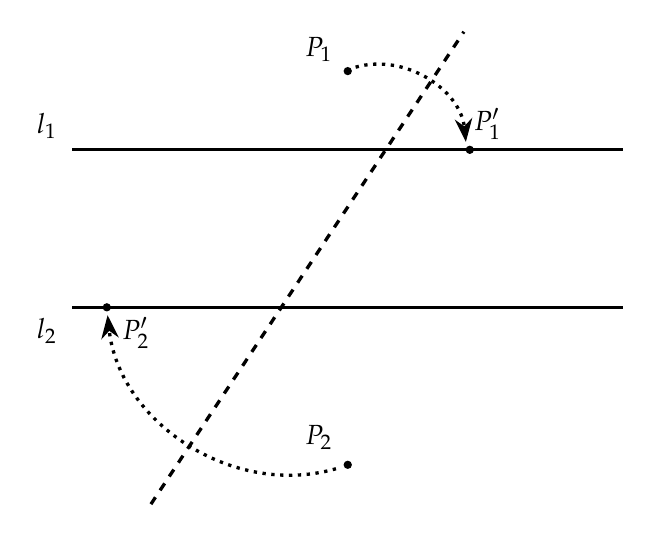
\begin{tikzpicture}[scale=.5]
\coordinate (P1) at (0,4);
\fill (P1) circle (3pt) node[above left,xshift=-2pt] {$P_1$};
\coordinate (P2) at (0,-6);
\fill (P2) circle (3pt) node[above left,xshift=-2pt,yshift=2pt] {$P_2$};
\coordinate (P1P) at (3.1,2);
\fill (P1P) circle (3pt) node[above right,xshift=-2pt] {$P_1'$};
\coordinate (P2P) at (-6.12,-2);
\fill (P2P) circle (3pt) node[below right,xshift=2pt] {$P_2'$};
\draw[very thick] (-7,2) -- node[very near start,above,xshift=-34pt] {$l_1$} (7,2);
\draw[very thick] (-7,-2) -- node[very near start,below,xshift=-34pt] {$l_2$} (7,-2);
\draw[very thick,dashed] (-5,-7) -- (2.95,5);
\draw[very thick,dotted,->,bend left=50] (.2,4.1) to (3,2.2);
\draw[very thick,dotted,->,bend left=50] (-.3,-6.1) to (-6.1,-2.2);
\end{tikzpicture}
\end{center}

\textbf{Axiom $7$} Given a point $P$ and two lines $l_1,l_2$, there is a fold that places $P$ onto $l_1$ and is perpendicular to $l_2$.

% Axiom 7
\begin{center}
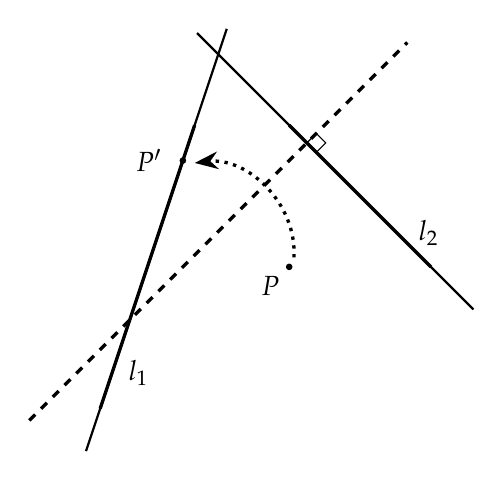
\begin{tikzpicture}[scale=.6]
\coordinate (P1) at (5,3);
\fill (P1) circle (2pt) node[below left] {$P$};
\coordinate (P1P) at (2.75,5.25);
\fill (P1P) circle (2pt) node[left,xshift=-4pt] {$P'$};
\draw[very thick] (1,0) -- node[very near start,right,xshift=2pt] {$l_1$} (3,6);
\draw[very thick,name path=l2] (8,3) -- node[very near start,right,xshift=-2pt,yshift=6pt] {$l_2$} (5,6);
\draw[thick] ($(1,0)!-.15!(3,6)$) -- ($(1,0)!1.34!(3,6)$);
\draw[thick] ($(8,3)!-.3!(5,6)$) -- ($(8,3)!1.65!(5,6)$);
\draw[very thick,dashed,name path=fold] (-.5,-.25) -- (7.5,7.75);
\path [name intersections = {of = fold and l2, by = {perp}}];
\draw[rotate=-45] (perp) rectangle +(8pt,8pt);
\draw[very thick,dotted,->,bend right=50] (5.1,3.2) to (3,5.2);
\end{tikzpicture}
\end{center}

%%%%%%%%%%%%%%%%%%%%%%%%%%%%%%%%%%%%%%%%%%%%%%%%%%%%%%%%%%%%%%%%%%
%%%%%%%%%%%%%%%%%%%%%%%%%%%%%%%%%%%%%%%%%%%%%%%%%%%%%%%%%%%%%%%%%%
%%%%%%%%%%%%%%%%%%%%%%%%%%%%%%%%%%%%%%%%%%%%%%%%%%%%%%%%%%%%%%%%%%

\subsection{The mathematics of origami}

The first axiom systems was \emph{Euclidean geometry}, named after the third-century mathematician who collected and extended geometrical theorems and proofs in the book \emph{The Elements}. Euclidean geometry was based on construction by straightedge (an unmarked ruler) and compass. The straightedge can construct a line that goes through two existing points; the compass can construct a circle from a given point (its center) and a given line segment (its radius).

There were three problems for which the Greeks were unable to find constructions with straightedge and compass: (1) trisecting an arbitrary angle into three equal parts; (2) squaring a circle: given a circle, construct a square with the same area; (3) doubling a cube: given a cube, construct another cube with twice the volume. In addition, they were unable to construct a regular heptagon (a regular polygon with seven sides).

It was not until the $19$-th century that the reason for their failures was understood. A straightedge and compass can only construct values that are obtainable from a line segment defined to have length $1$ and the operations of $\{+,-,\times, \div,\surd\}$. Squaring a circle is certainly impossible because it requires constructing the value $\pi$ which cannot be obtained from any algebraic formula. The other problems require the construction of cube roots which is impossible. For example, doubling a cube requires the construction of the value $\sqrt[3]{2}$.

The basic constructions of Euclidean geometry are: bisecting a line segment, bisecting an angle, copying a line segment, copying an angle, constructing a perpendicular to a line from a point not on the line, constructing a perpendicular to a line from a point on the line. All these constructions can be performed in origami using Axioms~$1$--$5$. The power of origami comes from Axiom~$6$: placing two points on two lines turns out to enable constructions that cannot be performed using straightedge and compass, in particular, constructions that require the computation of cube roots.

\subsection{Proof by folding}

Throughout the activities, the students will be asked to ``prove by folding.'' The intention is that the student perform a fold that will explain why a claim is true. Before each activity, the teacher must explain to the students when a fold proves a claim. We here present an example of a simple explanation that should be shown to the students before the activities (or as necessary).

% Axiom 2
\begin{wrapfigure}{r}{.4\textwidth}
\begin{center}
\vspace{-4ex}
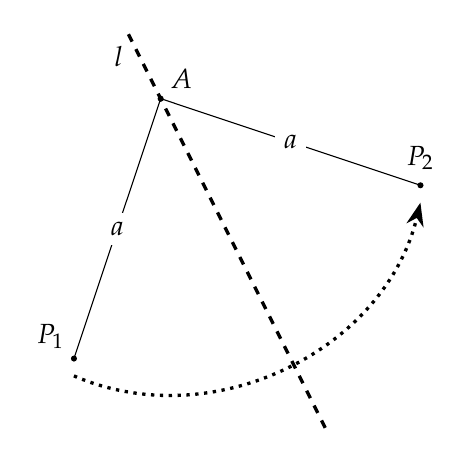
\begin{tikzpicture}[scale=1.1]
\coordinate (P1) at (2,2);
\coordinate (P2) at (6,4);
\coordinate (mid1) at ($(P1)!.5!(P2)$);
\coordinate (mid2) at ($(P1)!.5!(P2)+(-1,2)$);
\fill (mid2) circle(1pt) node[above right] {$A$};
\draw (P1) -- node[fill=white] {$a$} (mid2) -- node[fill=white] {$a$} (P2);
\draw[very thick,dashed] ($(mid1)!-.9!(mid2)$) --
  node[very near end,left,xshift=-6pt,yshift=8pt] {$l$}
  ($(mid1)!1.4!(mid2)$);
\fill (P1) circle(1pt) node[above left] {$P_1$};
\fill (P2) circle(1pt) node[above,yshift=2pt] {$P_2$};
\draw[very thick,dotted,->,bend right=50] (2,1.8) to (6,3.8);
\end{tikzpicture}
\end{center}	
\end{wrapfigure}
\textbf{Proof by folding}: Consider Axiom~$2$: given two points $P_1,P_2$, there is a single fold that places $P_1$ onto $P_2$. Look at the line constructed by this fold and an arbitrary point $A$ on the line. The fold does not move the point, so the line segment $\overline{AP_1}$ is placed onto the line segment $\overline{AP_2}$, so their lengths are equal. We have proved by folding that if the endpoints of a line segment are copied onto the endpoints of another segment then their lengths are equal.



\tikzsetfigurename{activities-locus}
% !TeX root = origami-activities-en.tex

%%%%%%%%%%%%%%%%%%%%%%%%%%%%%%%%%%%%%%%%%%%%%%%%%%%%%%%%%%%%%%%%%%
%%%%%%%%%%%%%%%%%%%%%%%%%%%%%%%%%%%%%%%%%%%%%%%%%%%%%%%%%%%%%%%%%%
%%%%%%%%%%%%%%%%%%%%%%%%%%%%%%%%%%%%%%%%%%%%%%%%%%%%%%%%%%%%%%%%%%

\section{Activities for learning geometric loci with origami}

\subsection{Introduction}

The activities are based on the origami axioms through which the students will experiment with constructing geometric loci. Paper folding can contribute to learning this concept because it provides a concrete visualization of the meaning of the concept.

\textbf{How to present the activities}

\begin{enumerate}

\item Each activity has two parts: in the first the students will get to know the axioms and the how the activities can be adapted for use in a classroom. The second part is a worksheet with the activity itself. Some students can be given the worksheets for independent study, while others may need to be guided through the steps of the activity.

\item The activities are arranged in an order that we believe is pedagogical optimal, not in the standard order of the axioms. Of course, the teacher is free to present the activities in a different order. Activity $1$ is essential to what follows and should be presented first, even if the teacher chooses a different order for the subsequent activities.

\item The activities include Geogebra applications intended to deepen the students' understanding of the geometric loci constructed by the axioms.
\end{enumerate}

\textbf{Paper for folding}

Several types of paper are appropriate for folding: (a) origami paper available in specialty shops; (b) any square or rectangular sheets of paper; (c) rectangular or square baking sheets which facilitate marking points and lines.

Each student should have at least six sheets of paper on hand (seven for the opening activity).

\subsection{The structure of an activity for leaning geometric loci}

\textbf{Topic} Geometric loci through paper folding.

\bigskip

\textbf{Goals} (a) Learning the concept and meaning of \emph{geometric locus} through paper folding; (b) learning the origami axioms; (c) exercising methods of finding geometric loci.

\bigskip

\textbf{Target audience} Secondary-school students studying advanced mathematics.

\bigskip

\textbf{Prerequisites} Analytic geometry with emphasis on circles and parabolas.

\newpage

\textbf{Structure}

\textbf{Part $1$}

\textbf{First phase: Acquaintance with origami}

\begin{enumerate}
\item The teacher will start with a brief presentation of the historical background of origami, describing how simple paper folding became an advanced mathematical theory and pioneering technological tool. At this point the students can be shown part of Robert Lang's lecture \cite{lang-ted}. Show four minutes starting from minute eleven.

\item The teacher will explain the origami axioms.

\item The teacher will acquaint the students with the basic concepts: point, line and fold.
\end{enumerate}

\textbf{Second phase: Familiarization and experimentation with the origami axioms} For the initial encounter with the axioms we suggest doing the activities described in Appendix~\ref{a.experimenting} \textit{Experimenting with folding according to the origami axioms}. 

\textbf{Third phase: Familiarization with the concept of geometric locus} The teacher will define the concept: the geometric locus is the set of points that satisfy a given condition. The locus is expressed as an expression of $y$ in terms of $x$. Often the locus can be expressed in geometric terms such as a point or line with a certain property, or a geometric figure like a circle or a parabola.

\bigskip

\textbf{Part $2$}

\textbf{First phase: Familiarization with geometric loci through the origami axioms} The teacher will distribute worksheets that ask the students to find geometric loci by paper folding (Section~\ref{s.discovery}). The students can work independently or work on each step followed by a group discussion.

\textbf{Second phase: Exercises} Section~\ref{s.exercises} contain mathematical exercises for each axiom. The first and second phases can be combined: at the conclusion of an activity from the first phase, the students can be asked to solve the respective exercise from the second phase.

\tikzsetfigurename{discovery-locus}
% !TeX root = origami-activities-en.tex

%%%%%%%%%%%%%%%%%%%%%%%%%%%%%%%%%%%%%%%%%%%%%%%%%%%%%%%%%%%%%%%%%%%
%%%%%%%%%%%%%%%%%%%%%%%%%%%%%%%%%%%%%%%%%%%%%%%%%%%%%%%%%%%%%%%%%%
%%%%%%%%%%%%%%%%%%%%%%%%%%%%%%%%%%%%%%%%%%%%%%%%%%%%%%%%%%%%%%%%%%

\section{Worksheets for the activities}\label{s.discovery}


In the following activities we investigate geometric loci through the origami axioms.

\subsection{The perpendicular bisector as a geometric locus}

% Axiom 2
\begin{wrapfigure}[4]{r}{.33\textwidth}
\begin{center}
\vspace{-10ex}
\begin{tikzpicture}[scale=.9]
\coordinate (P1) at (3,5);
\coordinate (P2) at (5,1);
\fill (P1) circle (1.5pt) node[above left] {$P_1$};
\fill (P2) circle (1.5pt) node[below right] {$P_2$};
\draw[thick,dashed] (2,2) -- (7,4);
\draw[very thick,dotted,->,bend left=35] (3.2,4.8) to (5,1.2);
\end{tikzpicture}
\end{center}
\end{wrapfigure}
Let us look at Axiom $2$: given two distinct points $P_1,P_2$, there is a single fold $l$ that places $P_1$ onto $P_2$. 

%\vspace{12ex}

Use a sheet of paper and perform the following operations:
\begin{itemize}
\item Choose two points and label them $P_1$ and $P_2$.
\item Fold the paper so that $P_1$ is placed onto $P_2$ and label the line created by the fold as $l$.
\item Choose an arbitrary point on $l$ and label it $A$.
\item Show by repeating the fold that $\overline{AP_1}=\overline{AP_2}$, that is, the distance of $A$ from $P_1$ equals the distance of $A$ from $P_2$.
\end{itemize}

\begin{center}
\begin{tikzpicture}[scale=1]
\coordinate (P1) at (2,2);
\coordinate (P2) at (6,4);
\coordinate (mid1) at ($(P1)!.5!(P2)$);
\coordinate (mid2) at ($(P1)!.5!(P2)+(-1,2)$);
\fill (mid2) circle(1pt) node[above right] {$A$};
\draw (P1) -- node[fill=white] {$a$} (mid2) -- node[fill=white] {$a$} (P2);
\draw[very thick,dashed] ($(mid1)!-1.4!(mid2)$) --
  node[very near end,left,xshift=-6pt,yshift=8pt] {$l$}
  ($(mid1)!1.4!(mid2)$);
\fill (P1) circle(1pt) node[above left] {$P_1$};
\fill (P2) circle(1pt) node[above,yshift=2pt] {$P_2$};
\draw[very thick,dotted,->,bend right=50] (2,1.8) to (6,3.8);
\end{tikzpicture}
\end{center}	

\begin{itemize}
\item Choose two more arbitrary points on $l$ and label them $B,C$.
\item Show by repeating the fold that $\overline{BP_1}=\overline{BP_2}$ and $\overline{CP_1}=\overline{CP_2}$.
\item What can you conclude about \emph{all} the points on the line $l$? The generalization is valid because $A,B,C$ were \emph{arbitrary} points on $l$.
\end{itemize}

\begin{center}
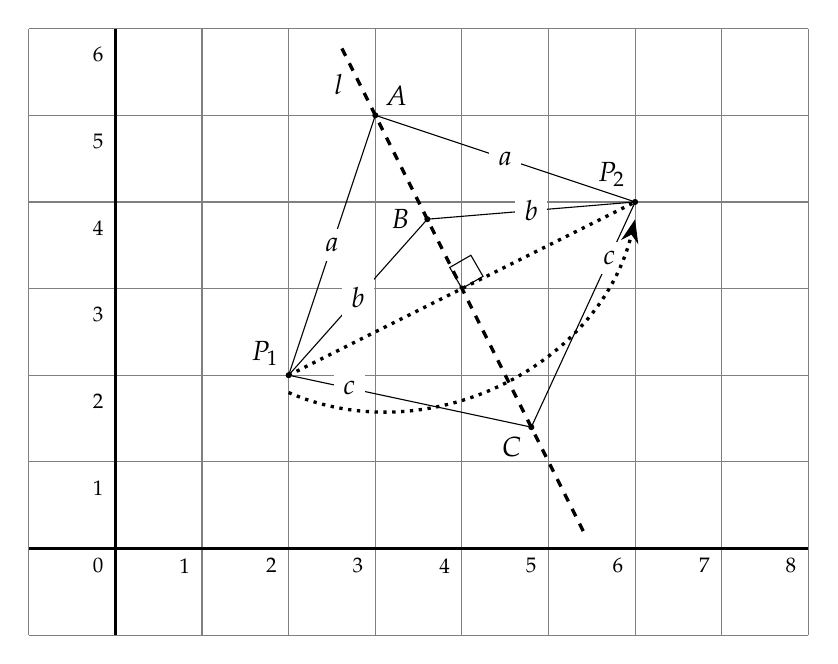
\begin{tikzpicture}[scale=1.1]
\draw[step=10mm,white!50!black,thin] (-1,-1) grid (8,6);
\draw[thick] (-1,0) -- (8,0);
\draw[thick] (0,-1) -- (0,6);
\foreach \x in {0,...,8}
  \node at (\x-.2,-.2) {\sm{\x}};
\foreach \y in {1,...,6}
  \node at (-.2,\y-.3) {\sm{\y}};
\coordinate (P1) at (2,2);
\coordinate (P2) at (6,4);
\coordinate (mid1) at ($(P1)!.5!(P2)$);
\coordinate (mid2) at ($(P1)!.5!(P2)+(-1,2)$);

\coordinate (mid3) at ($(mid1)!.4!(mid2)$);
\coordinate (mid4) at ($(mid1)!-.8!(mid2)$);

\fill (mid2) circle(1pt) node[above right] {$A$};
\fill (mid3) circle(1pt) node[left,xshift=-3pt] {$B$};
\fill (mid4) circle(1pt) node[below left] {$C$};

\draw (P1) -- node[fill=white] {$a$} (mid2) -- node[fill=white] {$a$} (P2);
\draw (P1) -- node[fill=white] {$b$} (mid3) -- node[fill=white] {$b$} (P2);
\draw (P1) -- node[fill=white,near start] {$c$} (mid4) -- 
  node[near end,fill=white] {$c$} (P2);

\draw[rotate=30] (mid1) rectangle +(8pt,8pt);

\draw[very thick,dotted] (P1) -- (P2);
\draw[very thick,dashed] ($(mid1)!-1.4!(mid2)$) --
  node[very near end,left,xshift=-6pt,yshift=8pt] {$l$}
  ($(mid1)!1.4!(mid2)$);
\fill (P1) circle(1pt) node[above left] {$P_1$};
\fill (P2) circle(1pt) node[above left,yshift=2pt] {$P_2$};

\draw[very thick,dotted,->,bend right=50] (2,1.8) to (6,3.8);
\end{tikzpicture}
\end{center}	

Open the Geogebra application for Axiom $1$ and move the slider so that the point moves on the fold---the red dashed line. Observe the distances of the points from the points $P_1,P_2$. The right angle and the distances are computed by Geogebra. What can you say about the distances? Do the results from the application support your conclusion from the previous paragraph?

Is it possible that there are points not on $l$ whose distance from $P_1$ is equal to its distance from $P_2$? Prove your claim. Hint: assume that such a point exists, label it $A'$ and derive a contradiction from the properties of the isoceles triangle $\triangle P_1A'P_2$.

What can we conclude about the geometric locus defined by $l$?

Prove that $l$ is the perpendicular bisector of $\overline{P_1P_2}$.

\begin{center}
\framebox[.9\textwidth]{\parbox{.85\textwidth}{
For all points $A$ on $l$, $\overline{AP_1}=\overline{AP_2}$.
$l$ is the perpendicular bisector of $\overline{P_1P_2}$ and therefore: \textbf{the geometric locus of all points equidistant from $P_1,P_2$ is the perpendicular bisector of $\overline{P_1P_2}$}.
}}
\end{center}

%%%%%%%%%%%%%%%%%%%%%%%%%%%%%%%%%%%%%%%%%%%%%%%%%%%%%%%%%%%%%%%%%%
%%%%%%%%%%%%%%%%%%%%%%%%%%%%%%%%%%%%%%%%%%%%%%%%%%%%%%%%%%%%%%%%%%
%%%%%%%%%%%%%%%%%%%%%%%%%%%%%%%%%%%%%%%%%%%%%%%%%%%%%%%%%%%%%%%%%%

\subsection{One and two lines as loci}


% Axiom 3
\begin{wrapfigure}{r}{.33\textwidth}
\begin{center}
\begin{tikzpicture}[scale=1]
\draw (1,2) -- node[near start,above,xshift=-4pt] {$l_1$} (3,6);
\draw (2,1) -- node[near start,below] {$l_2$} (7,3.5);
\draw[thick,dashed] (1,1) -- node[above] {$l$} (6,6);
\draw[very thick,dotted,->,bend left=35] (2.2,4.2) to (3.9,2.1);
\end{tikzpicture}
\end{center}
\end{wrapfigure}
Consider Axiom $3$: given two lines $l_1,l_2$ there are one or two folds that place $l_1$ onto $l_2$.


\textbf{Case $1$: $l_1,l_2$ intersect} 
\begin{itemize}
\item Draw two intersecting lines on a sheet of paper and label them $l_1$ and $l_2$. 
\item Fold the paper such that $l_1$ is placed onto $l_2$. Use a pen to mark the line created by the fold and label it $l$.
\item Choose an arbitrary point on $l$ and label it $A$.
\item Construct a perpendicular line from $A$ to $l_1$.
\item Prove by folding that the distance from $A$ to $l_1$ is equal to the distance from $A$ to $l_2$. Hint: First show that there are two triangles that are congruent by side-side-side and then use the properties of congruent triangles to prove the claim.
\item Can you prove the same claim for \emph{all} points on $l$? 
\end{itemize}

\begin{center}
\framebox[.9\textwidth]{\parbox{.85\textwidth}{
Every point on $l$ is equidistant from $l_1$ and $l_2$.
}}
\end{center}

\begin{center}
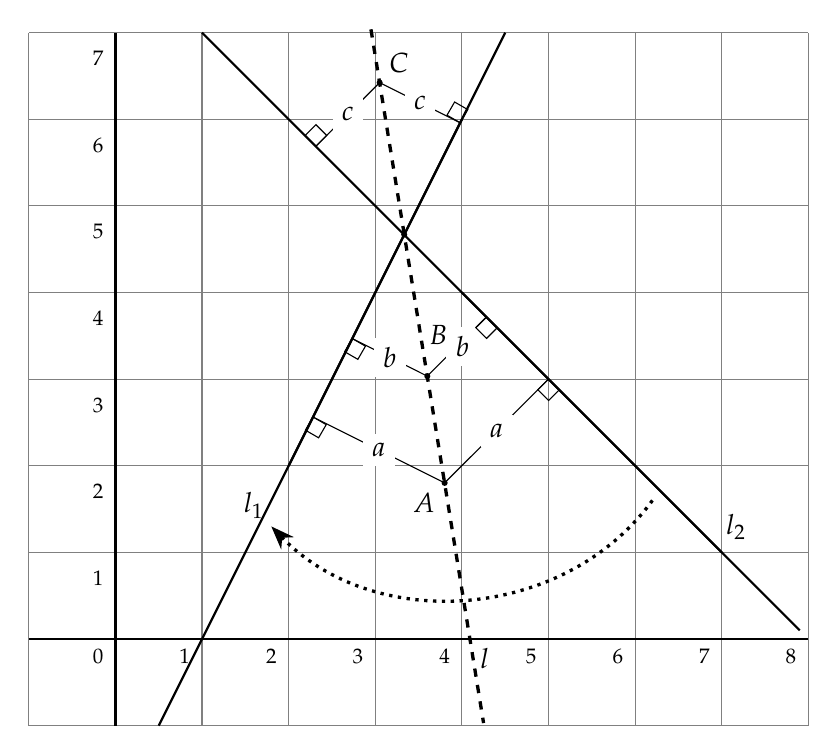
\begin{tikzpicture}[scale=1.1]
\draw[step=10mm,white!50!black,thin] (-1,-1) grid (8,7);
\draw[thick] (-1,0) -- (8,0);
\draw[thick] (0,-1) -- (0,7);
\foreach \x in {0,...,8}
  \node at (\x-.2,-.2) {\sm{\x}};
\foreach \y in {1,...,7}
  \node at (-.2,\y-.3) {\sm{\y}};
\coordinate (L1a) at (2,2);
\coordinate (L1b) at (4,6);
\draw[thick] (L1a) -- node[very near start,left,xshift=-13pt,yshift=-30pt] {$l_1$} (L1b);
\draw[thick,name path=l1] ($(L1a)!-.75!(L1b)$) -- ($(L1a)!1.25!(L1b)$);
\coordinate (L2a) at (7,1);
\coordinate (L2b) at (4,4);
\draw[thick] (L2a) -- (L2b);
\draw[thick,name path=l2] ($(L2a)!-.3!(L2b)$) -- node[very near start,above,xshift=4pt,yshift=2pt] {$l_2$} ($(L2a)!2!(L2b)$);
\path [name intersections = {of = l1 and l2, by = {PM}}];
\fill (PM) circle(1pt);

\coordinate (B2a) at (3,6.73);
\coordinate (B2b) at (4,.57);
\draw[very thick,dashed] ($(B2a)!-.05!(B2b)$) -- node[right,very near end,yshift=-8pt] {$l$}
  ($(B2a)!1.25!(B2b)$);

\draw[very thick,dotted,->,bend left=50] (6.2,1.6) to (1.8,1.3);

\coordinate (A) at ($(B2a)!.8!(B2b)$);
\fill (A) circle(1pt) node[below left] {$A$};
\coordinate (A1) at ($(PM)!(A)!(L2a)$);
\draw (A) -- node[fill=white] {$a$} (A1);
\draw[rotate=-135] (A1) rectangle +(5pt,5pt);
\coordinate (A2) at ($(PM)!(A)!(L1a)$);
\draw (A) -- node[fill=white] {$a$} (A2);
\draw[rotate=-120] (A2) rectangle +(5pt,5pt);

\coordinate (B) at ($(B2a)!.6!(B2b)$);
\fill (B) circle(1pt) node[above,xshift=4pt,yshift=8pt] {$B$};
\coordinate (B1) at ($(PM)!(B)!(L2a)$);
\draw (B) -- node[fill=white,xshift=2pt] {$b$} (B1);
\draw[rotate=-135] (B1) rectangle +(5pt,5pt);
\coordinate (B2) at ($(PM)!(B)!(L1a)$);
\draw (B) -- node[fill=white] {$b$} (B2);
\draw[rotate=-120] (B2) rectangle +(5pt,5pt);

\coordinate (C) at ($(B2a)!.05!(B2b)$);
\fill (C) circle(1pt) node[above right] {$C$};
\coordinate (C1) at ($(PM)!(C)!(L2a)$);
\draw (C) -- node[fill=white] {$c$} (C1);
\draw[rotate=45] (C1) rectangle +(5pt,5pt);
\coordinate (C2) at ($(PM)!(C)!(L1a)$);
\draw (C) -- node[fill=white] {$c$} (C2);
\draw[rotate=60] (C2) rectangle +(5pt,5pt);
\end{tikzpicture}
\end{center}

Open the Geogebra application for Axiom $3$. The size of the angles is computed by Geogebra. The perpendiculars from a point to the lines are labeled to check that the distances are equal. Experiment with the application. What property is satisfied by the fold?

Prove that $l$ bisects the vertical angles at the intersection of $l_1$ and $l_2$.

Can you find another fold that places $l_1$ onto $l_2$? If so, label it $l'$. What can you conclude about the points on $l'$?

Are there more folds that place $l_1$ onto $l_2$?

What is are the geometric loci represented by $l$ and $l'$?

\begin{center}
\framebox[.9\textwidth]{\parbox{.85\textwidth}{
The geometric loci of all points equidistant from two intersecting lines are the bisectors of the vertical angles at the point of intersection.
}}
\end{center}

\begin{center}
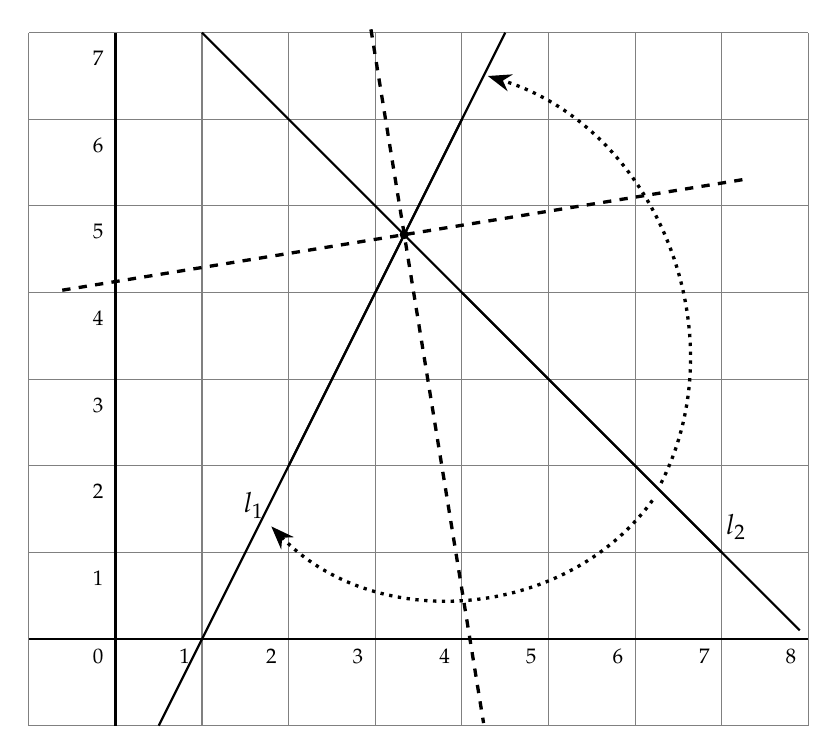
\begin{tikzpicture}[scale=1.1]
\draw[step=10mm,white!50!black,thin] (-1,-1) grid (8,7);
\draw[thick] (-1,0) -- (8,0);
\draw[thick] (0,-1) -- (0,7);
\foreach \x in {0,...,8}
  \node at (\x-.2,-.2) {\sm{\x}};
\foreach \y in {1,...,7}
  \node at (-.2,\y-.3) {\sm{\y}};
\coordinate (L1a) at (2,2);
\coordinate (L1b) at (4,6);
\draw[thick] (L1a) -- node[very near start,left,xshift=-13pt,yshift=-30pt] {$l_1$} (L1b);
\draw[thick,name path=l1] ($(L1a)!-.75!(L1b)$) -- ($(L1a)!1.25!(L1b)$);
\coordinate (L2a) at (7,1);
\coordinate (L2b) at (4,4);
\draw[thick] (L2a) -- (L2b);
\draw[thick,name path=l2] ($(L2a)!-.3!(L2b)$) -- node[very near start,above,xshift=4pt,yshift=2pt] {$l_2$} ($(L2a)!2!(L2b)$);
\path [name intersections = {of = l1 and l2, by = {PM}}];
\fill (PM) circle(1.5pt);
\coordinate (B2a) at (3,6.73);
\coordinate (B2b) at (4,.57);
\draw[very thick,dashed] ($(B2a)!-.05!(B2b)$) --
  ($(B2a)!1.25!(B2b)$);
\draw[very thick,dashed] ($(PM)!-4cm!90:(B2b)$) -- ($(PM)!4cm!90:(B2b)$);
\draw[very thick,dotted,->,bend left=50] (6.2,1.6) to (1.8,1.3);
\draw[very thick,dotted,->,bend right=50] (6.3,1.8) to (4.3,6.5);
\end{tikzpicture}
\end{center}

\textbf{Case $2$: $l_1$ is parallel to $l_2$}
\begin{itemize}
\item Draw two parallel lines on a sheet of paper and label them $l_1$ and $l_2$.
\item Fold the paper so that $l_1$ is placed onto $l_2$ and label the line constructed by the fold $l$.
\item Are there additional folds that place $l_1$ onto $l_2$?
\item Characterize the geometric locus of $l$. Hint: Choose a point $A$ on $l$ and show that it is equidistant from $l_1$ and $l_2$.
\end{itemize}
\begin{center}
\framebox[.9\textwidth]{\parbox{.85\textwidth}{
The geometric loci is a line parallel to $l_1$ and $l_2$ and equidistant from them.
}}
\end{center}

\begin{center}
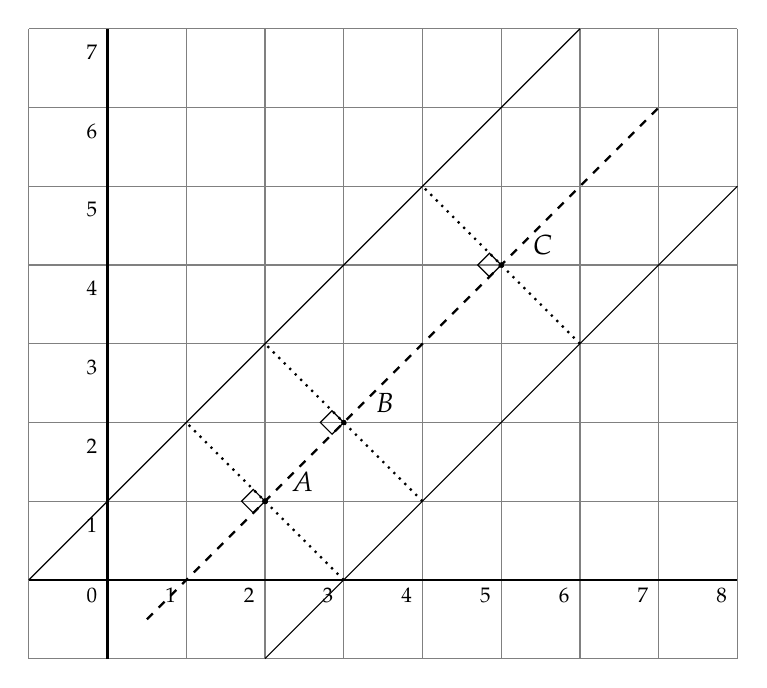
\begin{tikzpicture}[scale=1]
\draw[step=10mm,white!50!black,thin] (-1,-1) grid (8,7);
\draw[thick] (-1,0) -- (8,0);
\draw[thick] (0,-1) -- (0,7);
\foreach \x in {0,...,8}
  \node at (\x-.2,-.2) {\sm{\x}};
\foreach \y in {1,...,7}
  \node at (-.2,\y-.3) {\sm{\y}};
\draw (-1,0) -- (6,7);
\draw (2,-1) -- (8,5);
\draw[thick,dashed] (.5,-.5) -- (7,6);
\draw[thick,dotted] (3,0) -- (1,2);
\draw[thick,dotted] (4,1) -- (2,3);
\draw[thick,dotted] (6,3) -- (4,5);
\coordinate (A) at (2,1);
\node[above right,xshift=6pt] at (A) {$A$};
\coordinate (B) at (3,2);
\node[above right,xshift=8pt] at (B) {$B$};
\coordinate (C) at (5,4);
\node[above right,xshift=8pt] at (C) {$C$};
\fill (A) circle (1.1pt);
\fill (B) circle (1pt);
\fill (C) circle (1pt);
\draw[rotate=135] (A) rectangle +(6pt,6pt);
\draw[rotate=135] (B) rectangle +(6pt,6pt);
\draw[rotate=135] (C) rectangle +(6pt,6pt);
\end{tikzpicture}
\end{center}

%%%%%%%%%%%%%%%%%%%%%%%%%%%%%%%%%%%%%%%%%%%%%%%%%%%%%%%%%%%%%%%%%%
%%%%%%%%%%%%%%%%%%%%%%%%%%%%%%%%%%%%%%%%%%%%%%%%%%%%%%%%%%%%%%%%%%
%%%%%%%%%%%%%%%%%%%%%%%%%%%%%%%%%%%%%%%%%%%%%%%%%%%%%%%%%%%%%%%%%%

\subsection{A locus that is a line segment}

\begin{wrapfigure}[6]{r}{.33\textwidth}
% Axiom 1
\begin{center}
\vspace{-3ex}
\begin{tikzpicture}[scale=.9]
\coordinate (P1) at (3,6);
\coordinate (P2) at (4,3);
\fill (P1) circle (1.5pt) node[below left] {$P_1$};
\fill (P2) circle (1.5pt) node[below left] {$P_2$};
\draw[thick,dashed] ($(P1)!-.2!(P2)$) -- ($(P1)!1.5!(P2)$);
\draw[very thick,dotted,->,bend left=35] (5,5) to (2,4);
\end{tikzpicture}
\end{center}
\end{wrapfigure}
Consider Axiom 1: Given two points $P_1,P_2$, there is a single fold $l$ that passes through both points. 

Take a sheet of paper and perform the following operations:
\begin{itemize}
\item Choose two points and label them $P_1,P_2$.
\item Construct a fold that passes through both points.
\item Mark the line constructed by the fold and label it $l$.
\end{itemize}

Let us consider first only points that lie on the line segment $\overline{P_1P_2}$. Try to express a properties that characterizes all the points on the segment. Hint: Choose an arbitrary point on $\overline{P_1P_2}$. What is the sum of the distances from $P_1$ and $P_2$?

Are there other points in the plane not on $\overline{P_1P_2}$ that satisfy the same property? Justify your answer. Hint: The sum of the length of two sides of a triangle is always greater than the length of the third.

\begin{center}
\framebox[.9\textwidth]{\parbox{.85\textwidth}{
For an arbitrary point $A$ on $\overline{P_1P_2}$, $\overline{P_1P_2}= \overline{P_1A}+\overline{AP_2}$.
}}
\end{center}

\begin{center}
\framebox[.9\textwidth]{\parbox{.85\textwidth}{
The line segment $\overline{P_1P_2}$ is the geometric locus of all points the sum of whose distances from $P_1$ and $P_2$ is equal to the length of $\overline{P_1P_2}$.
}}
\end{center}

\begin{center}
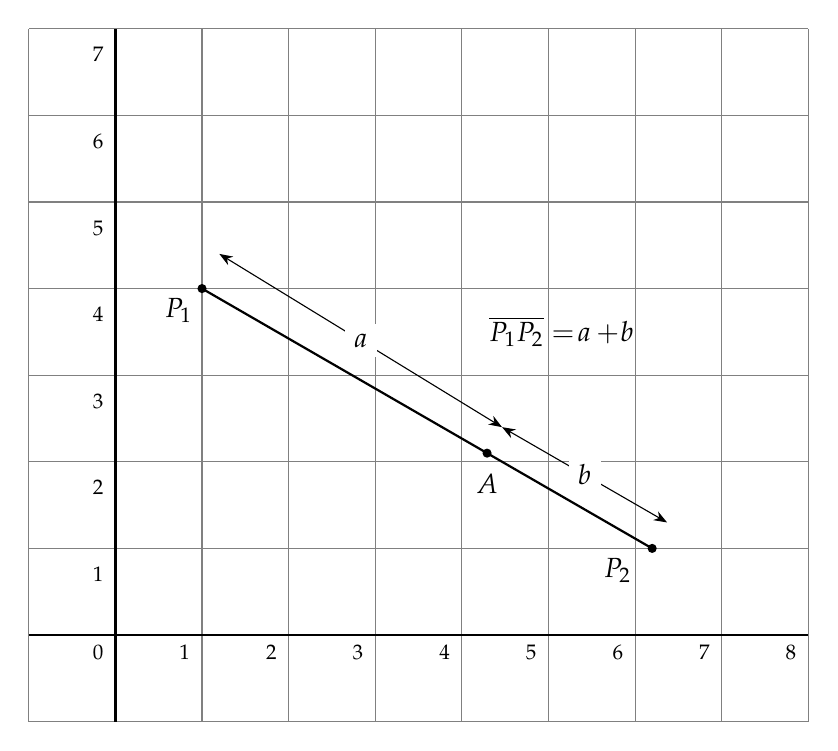
\begin{tikzpicture}[scale=1.1]
\draw[step=10mm,white!50!black,thin] (-1,-1) grid (8,7);
\draw[thick] (-1,0) -- (8,0);
\draw[thick] (0,-1) -- (0,7);
\foreach \x in {0,...,8}
  \node at (\x-.2,-.2) {\sm{\x}};
\foreach \y in {1,...,7}
  \node at (-.2,\y-.3) {\sm{\y}};
\coordinate (P1) at (1,4);
\coordinate (P2) at ($(P1)+(-30:6)$);
\fill (P1) circle (1.5pt) node[below left] {$P_1$};
\fill (P2) circle (1.5pt) node[below left,xshift=-4pt] {$P_2$};
\draw[thick] (P1) -- (P2);
%\draw[thick,dashed] ($(P1)!-.4!(P2)$) -- ($(P1)!1.4!(P2)$);
\draw[<->] ($(P1)+(.2,.4)$) -- node[fill=white] {$a$} ($(P1)+(0,.4)+(-30:4)$);
\draw[<->] ($(P1)+(0,.4)+(-30:4)$) -- node[fill=white] {$b$}  ($(P1)+(0,.4)+(-30:6.2)$);
\node at (5.15,3.5) {$\overline{P_1P_2}=\!a+\!b$};
\fill ($(P1)+(-30:3.8)$) circle(1.5pt) node[below,yshift=-4pt] {$A$};
\end{tikzpicture}
\end{center}

Consider now the points on $l$ that are not on $\overline{P_1P_2}$. Try to find a property that characterizes all such points. Hint: Choose an arbitrary point $A$ on $l$ but not on $\overline{P_1P_2}$ and look at the difference between the lengths $\overline{AP_1}$ and $\overline{AP_2}$.

Are there other points on the plane not on $l$ that satisfy this property? Hint: The sum of the length of two sides of any triangle is always greater than the length of the third side.

\begin{center}
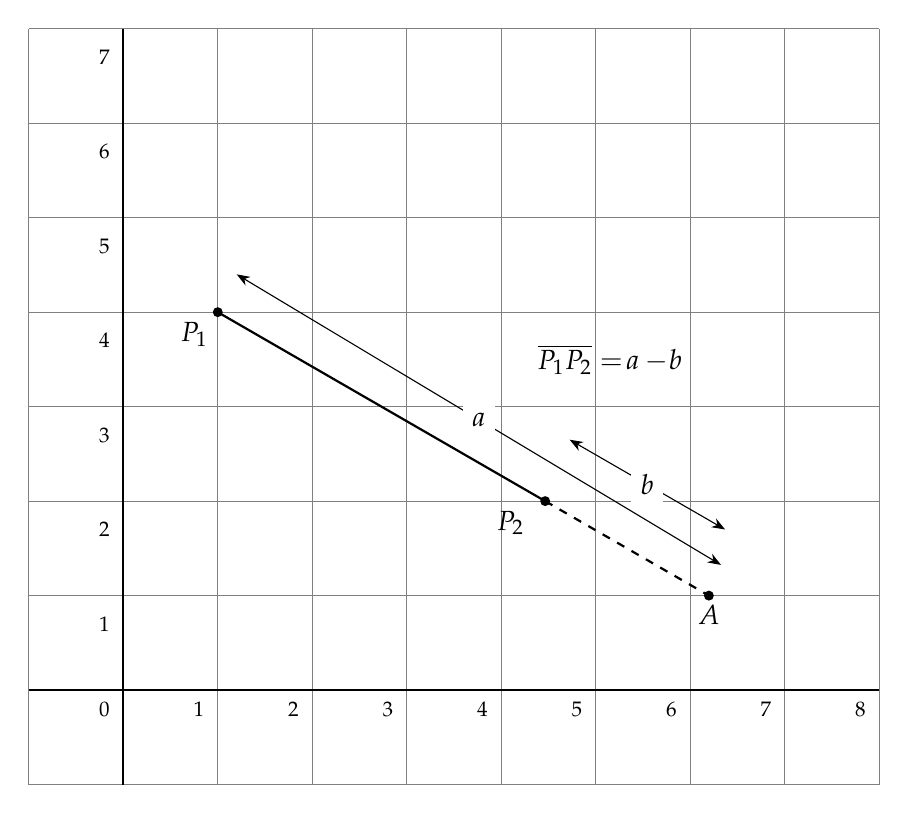
\begin{tikzpicture}[scale=1.2]
\draw[step=10mm,white!50!black,thin] (-1,-1) grid (8,7);
\draw[thick] (-1,0) -- (8,0);
\draw[thick] (0,-1) -- (0,7);
\foreach \x in {0,...,8}
  \node at (\x-.2,-.2) {\sm{\x}};
\foreach \y in {1,...,7}
  \node at (-.2,\y-.3) {\sm{\y}};
\coordinate (P1) at (1,4);
\coordinate (P2) at ($(P1)+(-30:4)$);
\fill (P1) circle (1.5pt) node[below left] {$P_1$};
\fill (P2) circle (1.5pt) node[below left,xshift=-4pt] {$P_2$};
\draw[thick] (P1) -- (P2);
\coordinate (p) at ($(P1)+(-30:6)$);
\draw[thick,dashed] (P2) -- (p);
\fill (p) circle (1.5pt) node[below] {$A$};
%\draw[thick,dashed] ($(P1)!-.4!(P2)$) -- ($(P1)!1.4!(P2)$);
\draw[<->] ($(P1)+(.2,.4)$) -- node[fill=white] {$a$} ($(P1)+(0,.4)+(-30:6.15)$);
\draw[<->] ($(P1)+(0,.8)+(-30:4.3)$) -- node[fill=white] {$b$}  ($(P1)+(0,.8)+(-30:6.2)$);
\node at (5.15,3.5) {$\overline{P_1P_2}=\!a-\!b$};
\end{tikzpicture}
\end{center}

We have found two properties one of which is satisfied by every point on $l$. Can you characterize the geometric locus defined by $l$?

\begin{center}
\framebox[.9\textwidth]{\parbox{.85\textwidth}{
\textbf{Conclusion}\\
$l$, the line constructed by the fold, is the geometric locus of all points $A$ such that the sum or difference of the lengths of $A$ from $P_1$ and $P_2$ is equal to the length of $\overline{P_1P_2}$.
}}
\end{center}
%%%%%%%%%%%%%%%%%%%%%%%%%%%%%%%%%%%%%%%%%%%%%%%%%%%%%%%%%%%%%%%%%%
%%%%%%%%%%%%%%%%%%%%%%%%%%%%%%%%%%%%%%%%%%%%%%%%%%%%%%%%%%%%%%%%%%
%%%%%%%%%%%%%%%%%%%%%%%%%%%%%%%%%%%%%%%%%%%%%%%%%%%%%%%%%%%%%%%%%%

\subsection{Loci appearing in Axiom 5}

\subsubsection{The circle as a locus}


\begin{wrapfigure}[5]{r}{.33\textwidth}
\begin{center}
\vspace{-6ex}
\begin{tikzpicture}[scale=1]
\coordinate (P1) at (1,4);
\coordinate (P2) at (4,3);
\fill (P1) circle (1.5pt) node[above left] {$P_1$};
\fill (P2) circle (1.5pt) node[below right] {$P_2$};
\draw[very thick,dotted] (P1) -- node[fill=white] {$a$} (P2);
\draw[thick,dashed] (0,1) -- (5,3.5);
\coordinate (P1a) at (3,0);
\fill (P1a) circle (1.5pt) node[below right,yshift=-2pt] {$P_1'$};
\draw[very thick, dotted] (P2) -- node[fill=white] {$a$} (P1a);
\draw[very thick,dotted,bend right=30,->] ($(P1)+(-.1,-.2)$) to ($(P1a)+(-.2,.1)$);
\end{tikzpicture}
\end{center}
\end{wrapfigure}
Take a sheet of paper and perform the following actions:
\begin{itemize}
\item Mark two points $P_1,P_2$.
\item Construct a fold through $P_2$ but don't open the paper.
\item Mark the point $P_1'$ that $P_1$ lands on. Tip: make a hole through the paper at $P_1$ to simplify marking $P_1'$.
\item Explain why the distance from $P_1$ to $P_2$ is equal to the distance from $P_1'$ to $P_2$ (both are labeled $a$ in the diagram).
\item Open the paper and perform the actions again and again with  different folds.
\end{itemize}
What is the common property of all the new points that are constructed?
\begin{center}
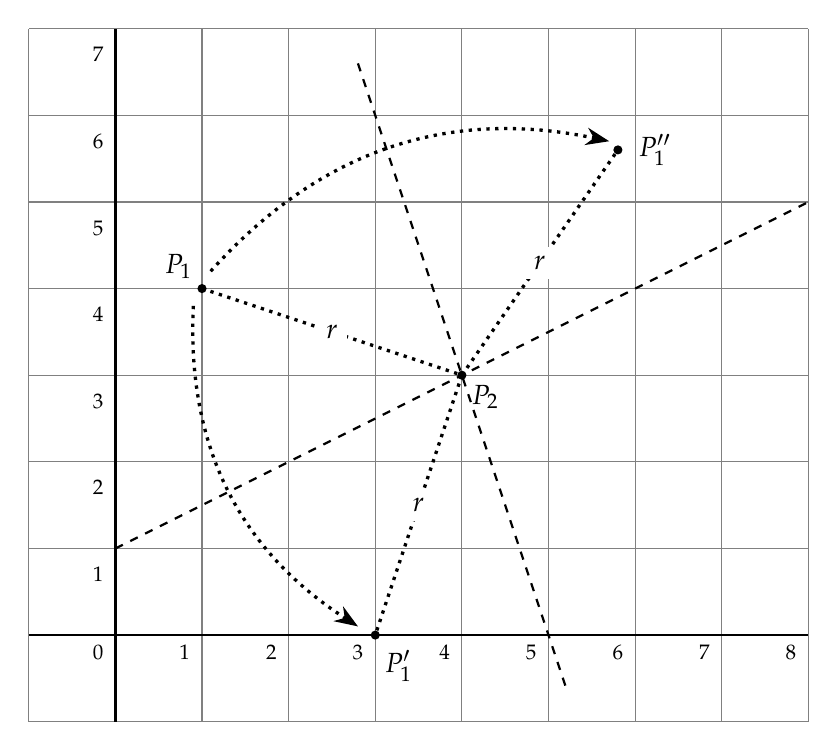
\begin{tikzpicture}[scale=1.1]
\draw[step=10mm,white!50!black,thin] (-1,-1) grid (8,7);
\draw[thick] (-1,0) -- (8,0);
\draw[thick] (0,-1) -- (0,7);
\foreach \x in {0,...,8}
  \node at (\x-.2,-.2) {\sm{\x}};
\foreach \y in {1,...,7}
  \node at (-.2,\y-.3) {\sm{\y}};
\coordinate (P1) at (1,4);
\coordinate (P2) at (4,3);
\fill (P1) circle (1.5pt) node[above left] {$P_1$};
\fill (P2) circle (1.5pt) node[below right] {$P_2$};
\draw[very thick,dotted] (P1) -- node[fill=white] {$r$} (P2);
\draw[thick,dashed] (0,1) -- (8,5);
\coordinate (P1a) at (3,0);
\fill (P1a) circle (1.5pt) node[below right,yshift=-2pt] {$P_1'$};
\draw[very thick, dotted] (P2) -- node[fill=white] {$r$} (P1a);
%\draw (P1) -- (P1a);
\draw[thick,dashed] ($(5,0)!1.1!(3,6)$) -- ($(3,6)!1.1!(5,0)$);
\coordinate (C) at ($(5,0)!(P1)!(3,6)$);
\coordinate (P1b) at ($(P1)!2!(C)$);
\fill (P1b) circle (1.5pt) node[right, xshift=4pt] {$P_1''$};
%\draw (P1) -- (P1b);
\draw[very thick,dotted] (P2) -- node[fill=white] {$r$} (P1b);
\draw[very thick,dotted,bend left=30,->] ($(P1)+(.1,.2)$) to ($(P1b)+(-.1,.1)$);
\draw[very thick,dotted,bend right=30,->] ($(P1)+(-.1,-.2)$) to ($(P1a)+(-.2,.1)$);
\end{tikzpicture}
\end{center}

\begin{center}
\framebox[.9\textwidth]{\parbox{.85\textwidth}{
All the points are the same distance from $P_2$; this distance is the length of $\overline{P_1P_2}$.
}}
\end{center}

Looking at the paper, what figure is formed by the new points?

Observe the Geogebra application called \texttt{circle.ggb}. Given points $P,Q$, the slider can be used to change the slope of the fold that passes through point $Q$. $P'$ is the reflection of point $P$ around the fold and its place will change as the slope of the fold is changed. If you check the box labeled ``Show trace of $P_1'$'', you can see all the reflected points.\footnote{The track can be erased by pressing ``Ctrl-F''.}
\begin{center}
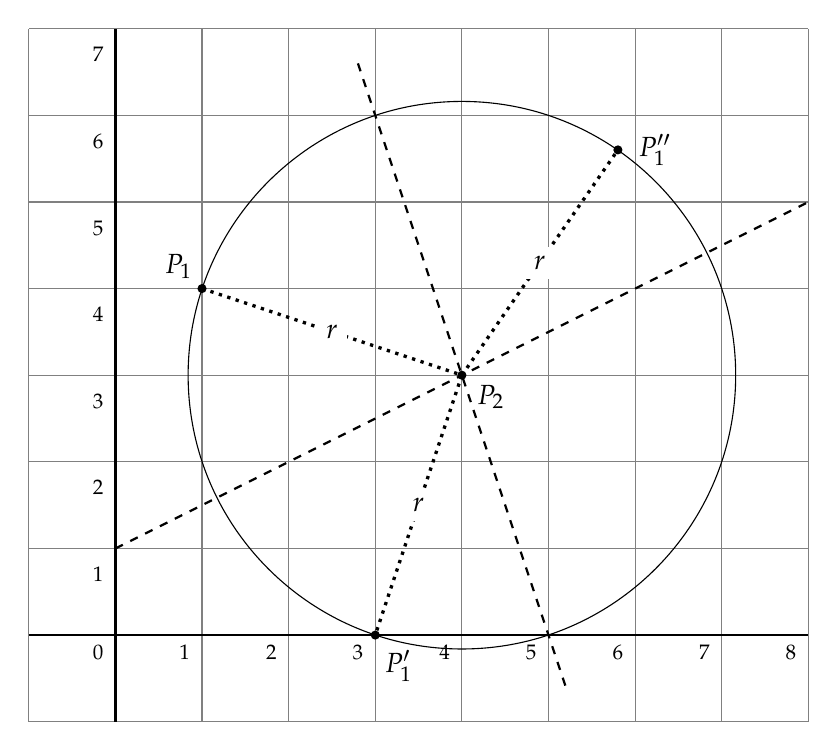
\begin{tikzpicture}[scale=1.1]
\draw[step=10mm,white!50!black,thin] (-1,-1) grid (8,7);
\draw[thick] (-1,0) -- (8,0);
\draw[thick] (0,-1) -- (0,7);
\foreach \x in {0,...,8}
  \node at (\x-.2,-.2) {\sm{\x}};
\foreach \y in {1,...,7}
  \node at (-.2,\y-.3) {\sm{\y}};
\coordinate (P1) at (1,4);
\coordinate (P2) at (4,3);
\fill (P1) circle (1.5pt) node[above left] {$P_1$};
\fill (P2) circle (1.5pt) node[below right,xshift=2pt] {$P_2$};
\draw[very thick,dotted] (P1) -- node[fill=white] {$r$} (P2);

\draw[thick,dashed] (0,1) -- (8,5);
\coordinate (P1a) at (3,0);
\fill (P1a) circle (1.5pt) node[below right,yshift=-2pt] {$P_1'$};
\draw[very thick, dotted] (P2) -- node[fill=white] {$r$} (P1a);
%\draw (P1) -- (P1a);
\draw[thick,dashed] ($(5,0)!1.1!(3,6)$) -- ($(3,6)!1.1!(5,0)$);
\coordinate (C) at ($(5,0)!(P1)!(3,6)$);
\coordinate (P1b) at ($(P1)!2!(C)$);
\fill (P1b) circle (1.5pt) node[right, xshift=4pt] {$P_1''$};
%\draw (P1) -- (P1b);
\draw[very thick,dotted] (P2) -- node[fill=white] {$r$} (P1b);
\node[draw,circle through=(P1)] at (P2) {};
\end{tikzpicture}
\end{center}
The reflected points form a circle. What is its center and radius? 

Could there be reflected points not on the circle, that is, inside or outside the circle? Explain.

What is the geometric locus of all points at a fixed distance from a given point?


\begin{center}
\framebox[.9\textwidth]{\parbox{.85\textwidth}{
The geometric locus of points at a fixed distance from a given point is a circle.
}}
\end{center}

%%%%%%%%%%%%%%%%%%%%%%%%%%%%%%%%%%%%%%%%%%%%%%%%%%%%%%%%%%%%%%%%%%
%%%%%%%%%%%%%%%%%%%%%%%%%%%%%%%%%%%%%%%%%%%%%%%%%%%%%%%%%%%%%%%%%%
%%%%%%%%%%%%%%%%%%%%%%%%%%%%%%%%%%%%%%%%%%%%%%%%%%%%%%%%%%%%%%%%%%

\subsubsection{Individual points are loci}

% Axiom 5
\begin{wrapfigure}[7]{r}{.33\textwidth}
\begin{center}
\vspace{-6ex}
\begin{tikzpicture}[scale=.8]
\coordinate (P1) at (1,4);
\coordinate (P2) at (4,3);
\fill (P1) circle (1.5pt) node[above left] {$P_1$};
\fill (P2) circle (1.5pt) node[below right] {$P_2$};
\draw[thick,dashed] (2.5,-1.5) -- (4.6,4.8); %($(3,0)!-.15!(5,6)$) -- (5,6);
\draw[thick] (1,-1) -- node[above] {$l$} ($(1,-1)!1.15!(7,2)$);
\coordinate (P3) at (7,2);
\fill (P3) circle (1.5pt) node[below right] {$P_1'$};
\draw[->,very thick,dotted,bend left=40] ($(P1)+(.2,.15)$) to ($(P3)+(-.2,.15)$);
\end{tikzpicture}
\end{center}
\end{wrapfigure}
Consider Axiom $5$: given two points $P_1,P_2$ and line $l$, there is a fold that places $P_1$ onto $l$ and passes through $P_2$.

Previously we saw that for any fold that passes through $P_2$, the possible reflections for $P_1$ form a circle whose center is $P_2$ and whose radius is the length of the line segment $\overline{P_1P_2}$. Axiom~$5$ adds a condition.

\begin{itemize}
\item What is the condition?
\item Of all the folds that constructed the circle, how may can possibly place $P_1$ onto the line $l$? There are three cases because the $l$ can intersect the circle in zero, one or two points. Use the Geogebra application to help answer this question.
\end{itemize}

\begin{center}
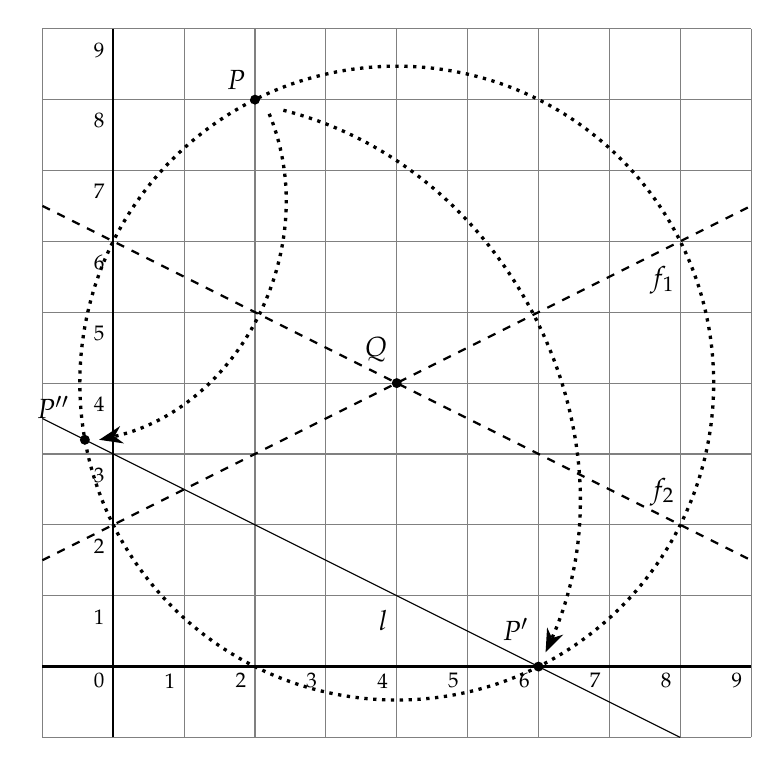
\begin{tikzpicture}[scale=.9]
\draw[step=10mm,white!50!black,thin] (-1,-1) grid (9,9);
\draw[thick] (-1,0) -- (9,0);
\draw[thick] (0,-1) -- (0,9);
\foreach \x in {0,...,9}
  \node at (\x-.2,-.2) {\sm{\x}};
\foreach \y in {1,...,9}
  \node at (-.2,\y-.3) {\sm{\y}};
\coordinate (L1a) at (-1,3.5);
\coordinate (L1b) at (8,-1);
\draw[name path=L1] (L1a) -- node[below,xshift=8pt,yshift=-8pt] {$l$} (L1b);
\coordinate (P1) at (2,8);
\fill (P1) circle (2pt) node[above left] {$P$};
\coordinate (P2) at (4,4);
\fill (P2) circle (2pt) node[above left,yshift=4pt] {$Q$};
\node[very thick,dotted,draw, name path = circle] at (P2)
    [circle through = (P1)] {};

\path [name intersections = {of = circle and L1, by = {P1P,P1PP}}];
\fill (P1P) circle (2pt) node[above left,xshift=-2pt,yshift=4pt] {$P''$};
\fill (P1PP) circle (2pt) node[above left,yshift=6pt] {$P'$};

\coordinate (f1) at (0,6);
\draw[thick,dashed] ($(f1)!-.25!(P2)$) -- node[very near end,above] {$f_2$} ($(f1)!2.25!(P2)$);
\coordinate (f2) at (0,2);
\draw[thick,dashed] ($(f2)!-.25!(P2)$) -- node[very near end,below,yshift=-2pt] {$f_1$} ($(f2)!2.25!(P2)$);

\draw[very thick,dotted,->,bend left=50] (2.2,7.8) to (-.2,3.2);
\draw[very thick,dotted,->,bend left=50] (2.4,7.85) to (6.1,.2);
\end{tikzpicture}
\end{center}
\textbf{Explanation of the Geogebra application} Given points $P,Q$ and line $l$, there are two folds $f_1,f_2$ through $Q$ that place $P$ onto $l$ at $P',P''$. In the previous application we saw that the geometric locus of the reflected points is a circle whose center is $Q$ and whose radius is the length of $\overline{PQ}$. The point $P',P''$ define the possible folds. Note that there will be no folds if the line $l$ does not intersect the circle and there will be one fold if the line is tangent to the circle.


Axiom $5$ describes the geometric locus of points on line $l$ whose distance from $P_2$ is the length of the line segment $\overline{P_1P_2}$. What is the form of the geometric locus in each of the cases described above?
\begin{center}
\framebox[.9\textwidth]{\parbox{.85\textwidth}{
Answers: Zero, one or two points depending on the number of intersections of $l$ with the circle formed by the points at distance $\overline{P_1P_2}$ from $P_2$.
}}
\end{center}

%%%%%%%%%%%%%%%%%%%%%%%%%%%%%%%%%%%%%%%%%%%%%%%%%%%%%%%%%%%%%%%%%%
%%%%%%%%%%%%%%%%%%%%%%%%%%%%%%%%%%%%%%%%%%%%%%%%%%%%%%%%%%%%%%%%%%
%%%%%%%%%%%%%%%%%%%%%%%%%%%%%%%%%%%%%%%%%%%%%%%%%%%%%%%%%%%%%%%%%%

\subsection{Loci appearing in Axiom 6}

\subsubsection{The parabola as a locus}

\begin{wrapfigure}[2]{r}{.4\textwidth}
\begin{center}
\vspace{-6ex}
\begin{tikzpicture}[scale=.8]
\draw[ultra thick] (0,0) -- node[above, near end] {$l$} (8,0);
\fill (3,3) circle (1.5pt) node[above left] {$P$};
\foreach \x in {1,2,5,7}
  \fill (\x,0) circle (1.5pt) node[above] {$P'$};
\end{tikzpicture}
\end{center}
\end{wrapfigure}
Take a sheet of paper and perform the following actions:
\begin{itemize}
\item Mark the line $l$ that is one edge of the paper.
\item Choose a point $P$ \emph{near} $l$ and a point $P'$ \emph{on} $l$.
\item Fold the paper so that $P'$ is place on $P$.
\item Open the paper and perform this action again and again for different positions of $P'$ on $l$.
\end{itemize}
Open the paper and observe the form created by the multiple folds. If necessary, perform additional folds until the form becomes clear.
\begin{center}
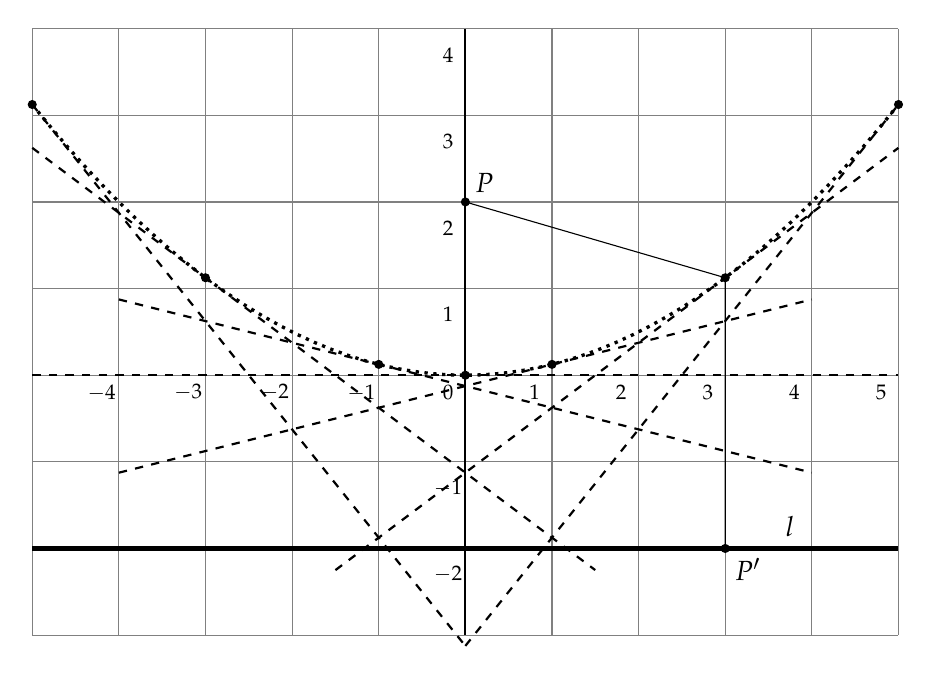
\begin{tikzpicture}[scale=1.1]
\draw[step=10mm,white!50!black,thin] (-2,-1) grid (8,6);
\draw[ultra thick] (-2,0) -- node[above, very near end] {$l$} (8,0);
\draw[thick,dashed] (-2,2) -- (8,2);
\draw[thick] (3,-1) -- (3,6);
\foreach \x in {-4,...,5}
  \node at (\x+3-.2,2-.2) {\sm{\x}};
\foreach \y in {-2,-1}
  \node at (3-.2,\y+2-.3) {\sm{\y}};
\foreach \y in {1,...,4}
  \node at (3-.2,\y+2-.3) {\sm{\y}};
\draw[domain=-5:5,samples=50,very thick,dotted,xshift=3cm,yshift=2cm] plot (\x,{(\x*\x)/8});
\coordinate (focus) at (3,4);
\fill (focus) circle(1.5pt) node[above right] {$P$};
\coordinate (pp) at (3+3,0);
\fill (pp) circle(1.5pt) node[below right] {$P'$};

\coordinate (p0) at (0+3,0+2);
\fill (p0) circle(1.5pt);
\coordinate (p1) at (1+3,.125+2);
\fill (p1) circle(1.5pt);
\coordinate (p3) at (3+3,1.125+2);
\fill (p3) circle(1.5pt);
\coordinate (p5) at (5+3,3.125+2);
\fill (p5) circle(1.5pt);

\draw (focus) -- (p3) -- (pp);


\coordinate (mp1) at (-1+3,.125+2);
\fill (mp1) circle(1.5pt);
\coordinate (mp3) at (-3+3,1.125+2);
\fill (mp3) circle(1.5pt);
\coordinate (mp5) at (-5+3,3.125+2);
\fill (mp5) circle(1.5pt);

\draw[domain=-4:4,samples=50,thick,dashed,xshift=3cm,yshift=2cm] plot (\x,{.125*(2*\x-1)});

\draw[domain=-1.5:5,samples=50,thick,dashed,xshift=3cm,yshift=2cm] plot (\x,{.375*(2*\x-3)});

\draw[domain=0:5,samples=50,thick,dashed,xshift=3cm,yshift=2cm] plot (\x,{.625*(2*\x-5)});

\draw[domain=-4:4,samples=50,thick,dashed,xshift=3cm,yshift=2cm] plot (\x,{-.125*(2*\x+1)});

\draw[domain=-5:1.5,samples=50,thick,dashed,xshift=3cm,yshift=2cm] plot (\x,{-.375*(2*\x+3)});

\draw[domain=-5:0,samples=50,thick,dashed,xshift=3cm,yshift=2cm] plot (\x,{-.625*(2*\x+5)});

\end{tikzpicture}
\end{center}
Use the Geogebra application \texttt{parabola.ggb} and select ``Show trace of $P$'' and move the slider to change the position of the point $P$. Then select ``Show locus'' to see the parabola formed by the positions of point $P$.

What do you think is the relationship between the folds and the parabola? Later we will prove that the folds are tangents to the parabola. 

Write down the definition of a parabola? Determine the focus and directrix for the parabola defined by the folds.


\textbf{How is the parabola formed?}
\begin{itemize}
\item Choose a point $P'$ on $l$ on the sheet of paper you have been using. Fold the paper so that $P'$ is placed onto $P$. Mark the line created by the fold and label it $l'$.
\item Construct a perpendicular to $l$ through the point $P'$. Label the intersection of the perpendicular and $l'$.
\item Show by folding that that $\overline{AP}=\overline{AP'}$. What can you conclude about the point $A$?
\end{itemize}
\begin{center}
\framebox[.9\textwidth]{\parbox{.85\textwidth}{
The distance of $A$ from $P$ is equal to the distance from $A$ to $l$. Therefore, $A$ is a point on the parabola whose focus is $P$ and whose directrix is $l$.
}}
\end{center}

\begin{center}
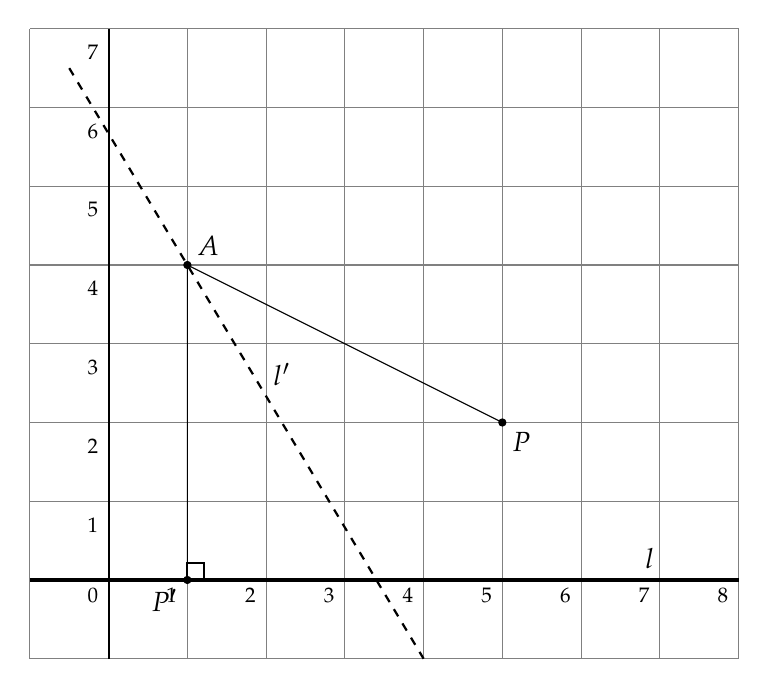
\begin{tikzpicture}[scale=1]
\draw[step=10mm,white!50!black,thin] (-1,-1) grid (8,7);
\draw[ultra thick] (-1,0) -- node[above, very near end] {$l$} (8,0);
\draw[thick] (0,-1) -- (0,7);
\foreach \x in {0,...,8}
  \node at (\x-.2,-.2) {\sm{\x}};
\foreach \y in {1,...,7}
  \node at (-.2,\y-.3) {\sm{\y}};
\coordinate (A) at (1,4);
\coordinate (P) at (5,2);
\coordinate (PP) at (1,0);
\fill (A) circle (1.5pt) node[above right] {$A$};
\fill (P) circle (1.5pt) node[below right] {$P$};
\fill (PP) circle (1.5pt) node[below left] {$P'$};
\draw (PP) -- (A) -- (P);
\draw[thick] (PP) rectangle +(6pt,6pt);
\draw[thick,dashed] ($(A)!-.5!(4,-1)$) -- node [right,xshift=6pt,yshift=-4pt] {$l'$} (4,-1);
\end{tikzpicture}
\end{center}

If we take into consideration all the possible folds, we obtain a parabola.
\begin{center}
\framebox[.9\textwidth]{\parbox{.85\textwidth}{
The geometric locus of all points equidistant from a given point (the focus) and a given line (the directrix) is a parabola.
}}
\end{center}

\begin{center}
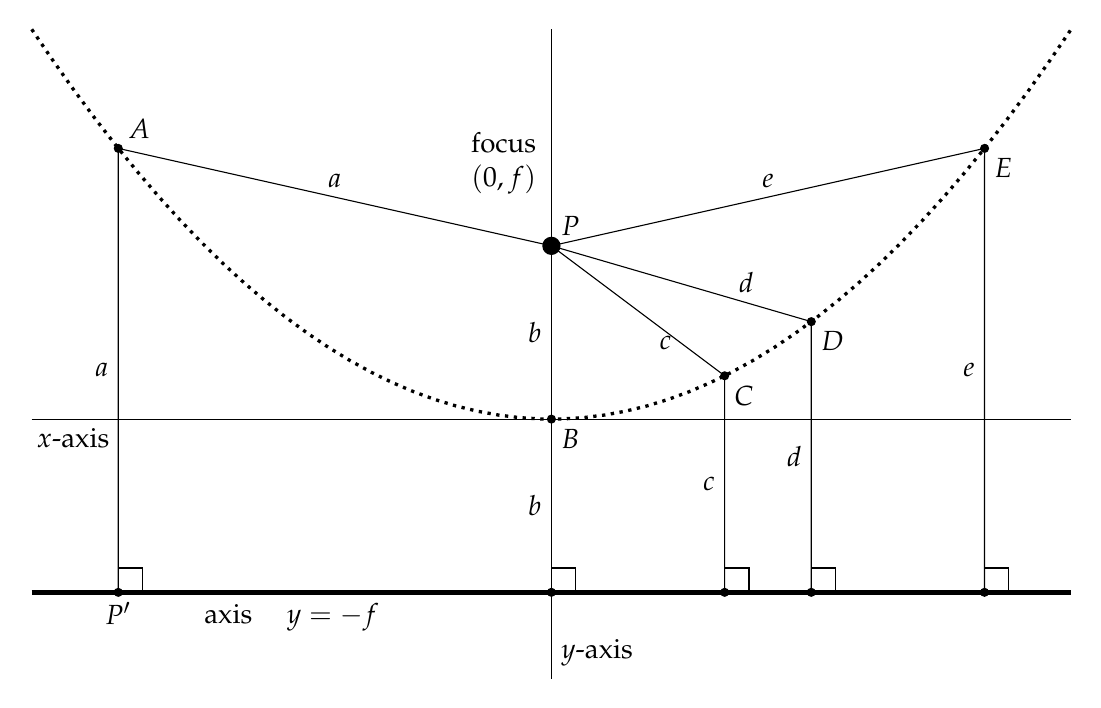
\begin{tikzpicture}[scale=1.1]
\draw (-6,0) -- node[very near start,below,xshift=-32pt] {$x$-axis} (6,0);
\draw (0,-3) -- node[very near start,right,yshift=-20pt] {$y$-axis} (0,4.5);
\draw[ultra thick] (-6,-2) -- node[near start,below] {axis $\quad y=-f$} (6,-2);
\draw[domain=-6:6,samples=50,very thick,dotted] plot (\x,{\x*\x/8});
\coordinate (F) at (0,2);
\fill (F) circle (3pt) node[above left,xshift=-2pt,yshift=15pt] {$(0,f)$} node[above left,xshift=-2pt,yshift=30pt] {focus} node[above right] {$P$};
\fill (0,0) circle (1.5pt) node[below right] {$B$};
\fill (0,-2) circle (1.5pt);
\fill (2,-2) circle (1.5pt);
\fill (3,-2) circle (1.5pt);
\fill (5,-2) circle (1.5pt);
\coordinate (FP) at (-5,-2);
\fill (FP) circle (1.5pt) node[below] {$P'$};
\coordinate (F1) at (2,.5);
\fill (F1) circle (1.5pt) node[below right] {$C$};
\coordinate (F2) at (3,1.125);
\fill (F2) circle (1.5pt) node[below right] {$D$};
\coordinate (F3) at (5,3.125);
\fill (F3) circle (1.5pt) node[below right] {$E$};
\coordinate (F4) at (-5,3.125);
\fill (F4) circle (1.5pt) node[above right] {$A$};
\draw (F) -- node[left] {$b$} (0,0) -- node[left] {$b$} (0,-2);
\draw (F) -- node[near end,left] {$c$} (F1) -- node[left] {$c$} (2,-2);
\draw (F) -- node[near end,above] {$d$} (F2) -- node[left] {$d$} (3,-2);
\draw (F) -- node[above] {$e$} (F3) -- node[left] {$e$} (5,-2);
\draw (F) -- node[above] {$a$} (F4) -- node[left] {$a$} (FP);
\draw (0,-2) rectangle +(8pt,8pt);
\draw (2,-2) rectangle +(8pt,8pt);
\draw (3,-2) rectangle +(8pt,8pt);
\draw (5,-2) rectangle +(8pt,8pt);
\draw (-5,-2) rectangle +(8pt,8pt);
\end{tikzpicture}
\end{center}

%%%%%%%%%%%%%%%%%%%%%%%%%%%%%%%%%%%%%%%%%%%%%%%%%%%%%%%%%%%%%%%%%%
%%%%%%%%%%%%%%%%%%%%%%%%%%%%%%%%%%%%%%%%%%%%%%%%%%%%%%%%%%%%%%%%%%
%%%%%%%%%%%%%%%%%%%%%%%%%%%%%%%%%%%%%%%%%%%%%%%%%%%%%%%%%%%%%%%%%%


\subsubsection{The tangent to a parabola}

Previously we saw that the set of folds that place a given point onto a given line forms a parabola. We now prove that each of these folds is a tangent to the parabola.
\begin{itemize}
\item Given a parabola with focus $P$ and directrix $l$, let $P'$ be a point on $l$. Prove that the fold that places $P$ onto $P'$ is the perpendicular bisector of the line segment $\overline{PP'}$. Hint: Prove that $\triangle APB \cong \triangle AP'B$.
\begin{center}
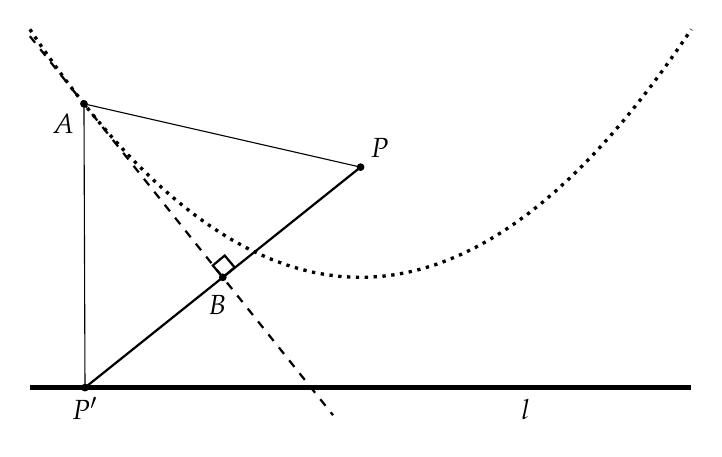
\begin{tikzpicture}[scale=.7]
\draw[ultra thick] (-6,-2) -- node[below,near end] {$l$}
(6,-2);
\draw[domain=-6:6,samples=50,very thick,dotted,name path=parb] plot (\x,{\x*\x/8});
\coordinate (F) at (0,2);
\fill (F) circle (2pt) node[above right] {$P$};
\coordinate (FP) at (-5,-2);
\fill (FP) circle (2pt) node[below] {$P'$};
\coordinate (F4) at (-5,3.125);
\draw[name path=perp,thick] (F) -- (FP);
\draw[thick,dashed,name path=fold] ($(F4)!-.4!(-2.5,0)$) --
($(F4)!1.8!(-2.5,0)$);
\path [name intersections = {of = fold and perp, by = {T}}];
\path [name intersections = {of = fold and parb, by = {Tan}}];
\fill (T) circle (2pt) node[below,xshift=-2pt,yshift=-3pt] {$B$};
\fill (Tan) circle (2pt) node[below left] {$A$};
\draw[thick,rotate=40] (T) rectangle +(8pt,8pt);
\draw (F) -- (Tan) -- (FP);
\end{tikzpicture}
\end{center}
\item Prove that the perpendicular bisector of the line segment connecting the focus with a point on the directrix is a tangent to the parabola.
\item Label the perpendicular bisector by $m$ and label its intersection with $\overline{PP'}$ by $B$.
\item Suppose that $m$ is not a tangent of the parabola. Then $m$ intersects the parabola in two different points, so there is a point $A'$ on $m$ that is distinct from $A$. Drop a perpendicular from $A'$ to $l$ and label its intersection with $l$ by $C$.
\item $A'$ is on the perpendicular bisector of $\overline{PP'}$ so $\overline{A'P}=\overline{A'P'}$ because $\triangle A'PB\cong \triangle A'P'B$.
\begin{center}
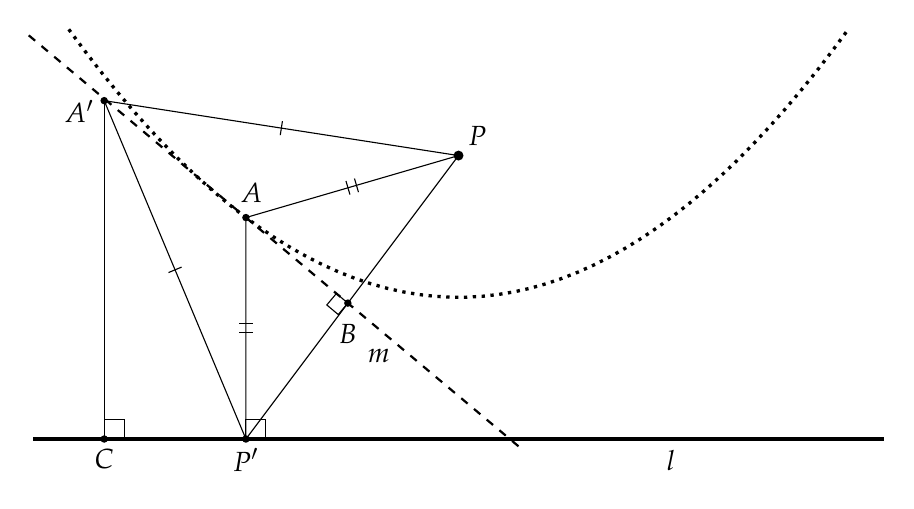
\begin{tikzpicture}[scale=.9]
\draw[ultra thick] (-6,-2) -- node[near end, below] {$l$} (6,-2);
\draw[domain=-5.5:5.5,samples=50,very thick,dotted] plot (\x,{\x*\x/8});
\coordinate (F) at (0,2);
\fill (F) circle (2pt) node[above right] {$P$};
\coordinate (FP) at (-3,-2);
\fill (FP) circle (1.5pt) node[below] {$P'$};
\coordinate (F4) at (-3,1.125);
\fill (F4) circle (1.5pt) node[above,yshift=2pt,xshift=2pt] {$A$};
\coordinate (F5) at (-5,2.775);
\fill (F5) circle (1.5pt) node[left,yshift=-4pt] {$A'$};
\coordinate (F5p) at (-5,-2);
\fill (F5p) circle (1.5pt) node[below] {$C$};
\draw (F) -- (F4) -- (FP);
%node[above] {$b$} (F4) -- node[left] {$b$} 
\draw (F) -- %node[above] {$c$} 
(F5);

\draw (F5) -- 
%node[left] {$d$}
 (F5p);
\draw[thick,dashed,name path=fold] ($(F4)+(140:4)$) -- (F4) -- node[below,xshift=-2pt,yshift=-2pt] {$m$} ($(F4)+(-40:5.1)$);
\draw (FP) rectangle +(8pt,8pt);
\draw (F5p) rectangle +(8pt,8pt);
\draw (F5) -- (FP);
\draw[name path=base] (F) -- (FP);
\path [name intersections = {of = base and fold, by = {G}}];
\fill (G) circle (1.5pt) node[below,yshift=-4pt] {$B$};
\draw[rotate=140] (G) rectangle +(6pt,6pt);
%\path (FP) -- node[left] {$c$} (F5);
%\path (F) -- node[below] {$a$} (G) -- node[below] {$a$} (FP);

% Draw tick marks
\coordinate(APP) at ($(F)!.5!(F5)$) ;
\draw (APP) -- ($(APP)!1mm!-90:(F)$);
\draw (APP) -- ($(APP)!1mm!90:(F)$);
\coordinate(APPP) at ($(F5)!.5!(FP)$) ;
\draw (APPP) -- ($(APPP)!1mm!-90:(F5)$);
\draw (APPP) -- ($(APPP)!1mm!90:(F5)$);

\coordinate(AP1) at ($(F)!.48!(F4)$) ;
\draw (AP1) -- ($(AP1)!1mm!-90:(F)$);
\draw (AP1) -- ($(AP1)!1mm!90:(F)$);
\coordinate(AP2) at ($(F)!.52!(F4)$) ;
\draw (AP2) -- ($(AP2)!1mm!-90:(F)$);
\draw (AP2) -- ($(AP2)!1mm!90:(F)$);

\coordinate(AAP1) at ($(F4)!.48!(FP)$) ;
\draw (AAP1) -- ($(AAP1)!1mm!-90:(F4)$);
\draw (AAP1) -- ($(AAP1)!1mm!90:(F4)$);
\coordinate(AAP2) at ($(F4)!.52!(FP)$) ;
\draw (AAP2) -- ($(AAP2)!1mm!-90:(F4)$);
\draw (AAP2) -- ($(AAP2)!1mm!90:(F4)$);
\end{tikzpicture}
\end{center}
\item $A'$ is on the parabola so $\overline{A'P}=\overline{A'C}$ and $l\perp \overline{A'C}$. It follows that $\overline{A'P'}=\overline{A'C}$.
\item It follows that in the right triangle $\triangle A'CP'$, the length of the side $\overline{A'C}$ is equal to the length of the hypotenuse $\overline{A'P'}$ which is impossible.
\item We conclude that $m$ cannot intersect the parabola in more than one point so it is a tangent to the parabola.
\end{itemize}

\begin{center}
\framebox[.9\textwidth]{\parbox{.85\textwidth}{
The perpendicular bisector of the line segment connecting the focus of a parabola and a point on the directrix is a tangent to the parabola.
}}
\end{center}

%%%%%%%%%%%%%%%%%%%%%%%%%%%%%%%%%%%%%%%%%%%%%%%%%%%%%%%%%%%%%%%%%%
%%%%%%%%%%%%%%%%%%%%%%%%%%%%%%%%%%%%%%%%%%%%%%%%%%%%%%%%%%%%%%%%%%
%%%%%%%%%%%%%%%%%%%%%%%%%%%%%%%%%%%%%%%%%%%%%%%%%%%%%%%%%%%%%%%%%%


\subsection{The locus described by Axiom 6}

% Axiom 6
\begin{wrapfigure}[8]{r}{.5\textwidth}
\begin{center}
\vspace{-8ex}
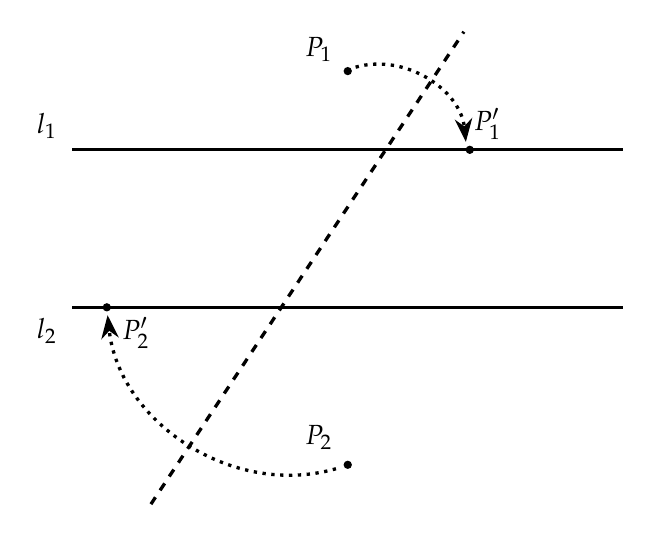
\begin{tikzpicture}[scale=.5]
\coordinate (P1) at (0,4);
\fill (P1) circle (3pt) node[above left,xshift=-2pt] {$P_1$};
\coordinate (P2) at (0,-6);
\fill (P2) circle (3pt) node[above left,xshift=-2pt,yshift=2pt] {$P_2$};
\coordinate (P1P) at (3.1,2);
\fill (P1P) circle (3pt) node[above right,xshift=-2pt] {$P_1'$};
\coordinate (P2P) at (-6.12,-2);
\fill (P2P) circle (3pt) node[below right,xshift=2pt] {$P_2'$};
\draw[very thick] (-7,2) -- node[very near start,above,xshift=-34pt] {$l_1$} (7,2);
\draw[very thick] (-7,-2) -- node[very near start,below,xshift=-34pt] {$l_2$} (7,-2);
\draw[very thick,dashed] (-5,-7) -- (2.95,5);
\draw[very thick,dotted,->,bend left=50] (.2,4.1) to (3,2.2);
\draw[very thick,dotted,->,bend left=50] (-.3,-6.1) to (-6.1,-2.2);
\end{tikzpicture}
\end{center}
\end{wrapfigure}
Consider Axiom $6$: Given two points $P_1,P_2$ and two lines $l_1,l_2$, there is a fold that places $P_1$ on $l_1$ and $P_2$ on $l_2$.

We saw that the set of folds that place a point $P$ on a line $l$ create a parabola. In addition we proved that each fold is a tangent to the parabola. Therefore, the folds that place $P_i$ on $l_i$, $i=1,2$ are the tangents to the parabolas whose foci are $P_i$ and whose directrices are $l_i$. 
%\begin{center}
%\begin{tikzpicture}[scale=1.2]
%\draw[step=10mm,white!50!black,thin] (-2,-1) grid (8,6);
%\draw[ultra thick] (-2,0) -- node[above, very near end] {$l$} (8,0);
%\draw[thick,dashed] (-2,2) -- (8,2);
%\draw[thick] (3,-1) -- (3,6);
%\foreach \x in {-4,...,5}
%  \node at (\x+3-.2,2-.2) {\sm{\x}};
%\foreach \y in {-2,-1}
%  \node at (3-.2,\y+2-.3) {\sm{\y}};
%\foreach \y in {1,...,4}
%  \node at (3-.2,\y+2-.3) {\sm{\y}};
%\draw[domain=-5:5,samples=50,very thick,dotted,xshift=3cm,yshift=2cm] plot (\x,{(\x*\x)/8});
%\coordinate (focus) at (3,4);
%\fill (focus) circle(1.5pt) node[above right] {$P$};
%\coordinate (pp) at (3+3,0);
%\fill (pp) circle(1.5pt) node[below right] {$P'$};
%\coordinate (p0) at (0+3,0+2);
%\fill (p0) circle(1.5pt);
%\coordinate (p1) at (1+3,.125+2);
%\fill (p1) circle(1.5pt);
%\coordinate (p3) at (3+3,1.125+2);
%\fill (p3) circle(1.5pt);
%\coordinate (p5) at (5+3,3.125+2);
%\fill (p5) circle(1.5pt);
%\draw (focus) -- (p3) -- (pp);
%\coordinate (mp1) at (-1+3,.125+2);
%\fill (mp1) circle(1.5pt);
%\coordinate (mp3) at (-3+3,1.125+2);
%\fill (mp3) circle(1.5pt);
%\coordinate (mp5) at (-5+3,3.125+2);
%\fill (mp5) circle(1.5pt);
%\draw[domain=-4:4,samples=50,thick,dashed,xshift=3cm,yshift=2cm] plot (\x,{.125*(2*\x-1)});
%\draw[domain=-1.5:5,samples=50,thick,dashed,xshift=3cm,yshift=2cm] plot (\x,{.375*(2*\x-3)});
%\draw[domain=0:5,samples=50,thick,dashed,xshift=3cm,yshift=2cm] plot (\x,{.625*(2*\x-5)});
%\draw[domain=-4:4,samples=50,thick,dashed,xshift=3cm,yshift=2cm] plot (\x,{-.125*(2*\x+1)});
%\draw[domain=-5:1.5,samples=50,thick,dashed,xshift=3cm,yshift=2cm] plot (\x,{-.375*(2*\x+3)});
%\draw[domain=-5:0,samples=50,thick,dashed,xshift=3cm,yshift=2cm] plot (\x,{-.625*(2*\x+5)});
%\end{tikzpicture}
%\end{center}

\newpage

How can a fold simultaneously satisfy these two conditions? 

The fold must be a tangent of both parabolas!

%\begin{wrapfigure}[8]{r}{.5\textwidth}
\begin{center}
%\vspace{-2ex}
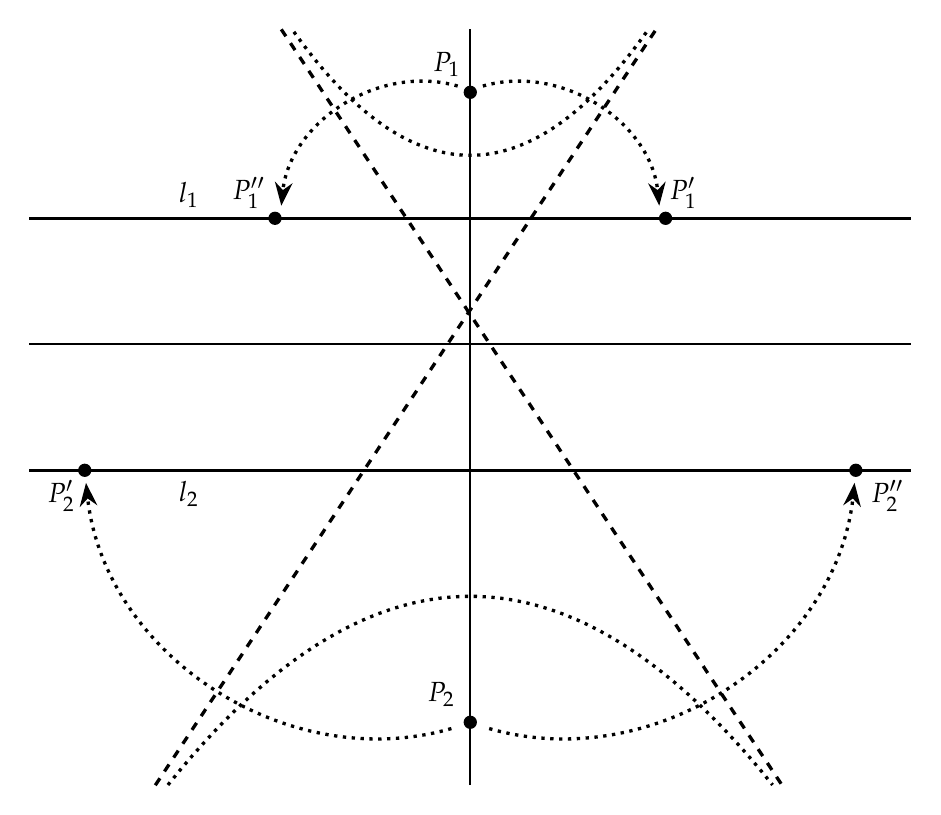
\begin{tikzpicture}[scale=.8]
\draw[thick] (-7,0) -- (7,0);
\draw[thick] (0,-7) -- (0,5);
\coordinate (P1) at (0,4);
\fill (P1) circle (3pt) node[above left,xshift=0pt,yshift=2pt] {$P_1$};
\coordinate (P2) at (0,-6);
\fill (P2) circle (3pt) node[above left,xshift=-2pt,yshift=2pt] {$P_2$};
\coordinate (P1P) at (3.1,2);
\fill (P1P) circle (3pt) node[above right,xshift=-2pt] {$P_1'$};
\coordinate (P2P) at (-6.12,-2);
\fill (P2P) circle (3pt) node[below left,xshift=0pt] {$P_2'$};
\coordinate (P1PP) at (-3.1,2);
\fill (P1PP) circle (3pt) node[above left,xshift=0pt] {$P_1''$};
\coordinate (P2PP) at (6.12,-2);
\fill (P2PP) circle (3pt) node[below right,xshift=2pt] {$P_2''$};
\draw[very thick] (-7,2) -- node[near start,above,xshift=-22pt] {$l_1$} (7,2);
\draw[very thick] (-7,-2) -- node[near start,below,xshift=-22pt] {$l_2$} (7,-2);
\draw[domain=-4.8:4.8,samples=50,very thick,dotted] plot (\x,{-.13*\x*\x-4});
\draw[domain=-2.8:2.8,samples=50,very thick,dotted] plot (\x,{.25*\x*\x+3});
\draw[very thick,dashed] (-5,-7) -- (2.95,5);
\draw[very thick,dashed] (-3,5) -- (4.95,-7);
\draw[very thick,dotted,->,bend left=50] (.2,4.1) to (3,2.2);
\draw[very thick,dotted,->,bend left=50] (-.3,-6.1) to (-6.1,-2.2);
\draw[very thick,dotted,->,bend right=50] (-.2,4.1) to (-3,2.2);
\draw[very thick,dotted,->,bend right=50] (.3,-6.1) to (6.1,-2.2);
\end{tikzpicture}
\end{center}
%\end{wrapfigure}
\begin{itemize}
\item Do all pairs of parabolas have a common tangent?
\item How many common tangents can a pair of parabolas have? See Appendix~\ref{a.parabola}.
\item What does it mean in terms of Axiom $6$ for a pair of parabolas to have more than one common tangent?
\end{itemize}
\begin{center}
\framebox[.9\textwidth]{\parbox{.85\textwidth}{
A fold resulting from Axiom $6$ is a common tangent to two parabolas with foci $P_1,P_1$ and directrices $l_1,l_2$.

Two parabolas can have zero, one, two or three common tangents.

Therefore, there can be zero, one, two or three folds satisfying Axiom 6 for any given $P_1, P_2, l_1, l_2$.
}}
\end{center}



%%%%%%%%%%%%%%%%%%%%%%%%%%%%%%%%%%%%%%%%%%%%%%%%%%%%%%%%%%%%%%%%%%
%%%%%%%%%%%%%%%%%%%%%%%%%%%%%%%%%%%%%%%%%%%%%%%%%%%%%%%%%%%%%%%%%%
%%%%%%%%%%%%%%%%%%%%%%%%%%%%%%%%%%%%%%%%%%%%%%%%%%%%%%%%%%%%%%%%%%

\subsection{The locus described by Axiom $4$}

\begin{wrapfigure}{r}{.4\textwidth}
% Axiom 4
\begin{center}
\vspace{-8ex}
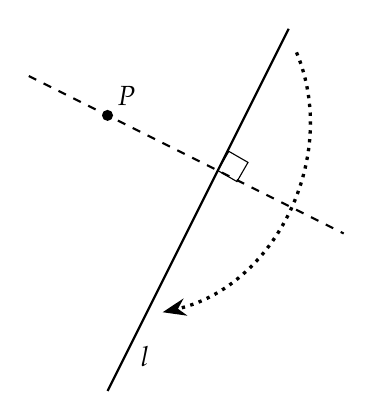
\begin{tikzpicture}[scale=1]
\coordinate (L1a) at (3,2);
\coordinate (L1b) at (5,6);
\draw[thick] (L1a) -- node[very near start,right,yshift=-4pt] {$l$} ($(L1a)!1.15!(L1b)$);
\fill (3,5.5) circle (2pt) node[above right] {$P$};
\draw[thick,dashed] (2,6) -- (6,4);
\coordinate (intersection) at (4.4,4.8);
\draw[rotate=-30] (intersection) rectangle +(8pt,8pt);
\draw[very thick,dotted,->,bend left=50] (5.4,6.3) to (3.7,3);
\end{tikzpicture}
\end{center}
\end{wrapfigure}
\textbf{Axiom $4$} Given a point $P$ and a line $l$, there is a single fold perpendicular to $l$ that passes through $P$.
\begin{itemize}
\item Take a sheet of paper and mark an arbitrary point $P$ and an arbitrary line $l$.
\item Fold the paper so that the fold is perpendicular to $l$ and passes through $P$.
\item What is the geometric locus of the fold?
\end{itemize}
\vspace{-2ex}
\begin{center}
\framebox[.9\textwidth]{\parbox{.85\textwidth}{
The fold created by Axiom $4$ is the geometric locus of all points on the line perpendicular to $l$ and passing through $P$.
}}
\end{center}

\bigskip

\subsection{The locus described by Axiom $7$}


% Axiom 7
\begin{wrapfigure}[4]{r}{.4\textwidth}
\begin{center}
\vspace{-6ex}
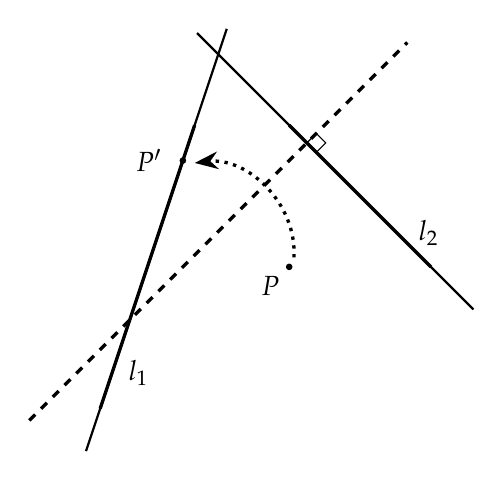
\begin{tikzpicture}[scale=.6]
\coordinate (P1) at (5,3);
\fill (P1) circle (2pt) node[below left] {$P$};
\coordinate (P1P) at (2.75,5.25);
\fill (P1P) circle (2pt) node[left,xshift=-4pt] {$P'$};
\draw[very thick] (1,0) -- node[very near start,right,xshift=2pt] {$l_1$} (3,6);
\draw[very thick,name path=l2] (8,3) -- node[very near start,right,xshift=-2pt,yshift=6pt] {$l_2$} (5,6);
\draw[thick] ($(1,0)!-.15!(3,6)$) -- ($(1,0)!1.34!(3,6)$);
\draw[thick] ($(8,3)!-.3!(5,6)$) -- ($(8,3)!1.65!(5,6)$);
\draw[very thick,dashed,name path=fold] (-.5,-.25) -- (7.5,7.75);
\path [name intersections = {of = fold and l2, by = {perp}}];
\draw[rotate=-45] (perp) rectangle +(8pt,8pt);
\draw[very thick,dotted,->,bend right=50] (5.1,3.2) to (3,5.2);
\end{tikzpicture}
\end{center}
\end{wrapfigure}
\textbf{Axiom $7$} Given a point $P$ and two lines $l_1,l_2$, there is a fold that places $P$ onto $l_1$ and is perpendicular to $l_2$.
\begin{itemize}
\item Take a sheet of paper and mark a point $P$ and two lines $l_1,l_2$.
\item Fold the paper as described in Axiom $7$: a fold perpendicular to $l_2$ that places $P$ onto $l_1$.
\item Leave the paper folded and mark the point upon which $P$ is placed by $P'$.
\item Open the paper.
\end{itemize}
Explain why every point on the fold is equidistant from $p$ and $P'$.
Hint: Recall from Axiom $2$ and the activities that its geometric locus is the perpendicular bisector. 

What characterizes the set of points on the fold created by Axiom $7$?

What is the geometric locus described by those points?

\begin{center}
\framebox[.9\textwidth]{\parbox{.85\textwidth}{
The fold created by Axiom $7$ is the geometric locus of all points on the line perpendicular to $l_2$ and equidistant from $P$ and $P'$, the reflection of $P$ onto $l_1$.
}}
\end{center}

\begin{center}
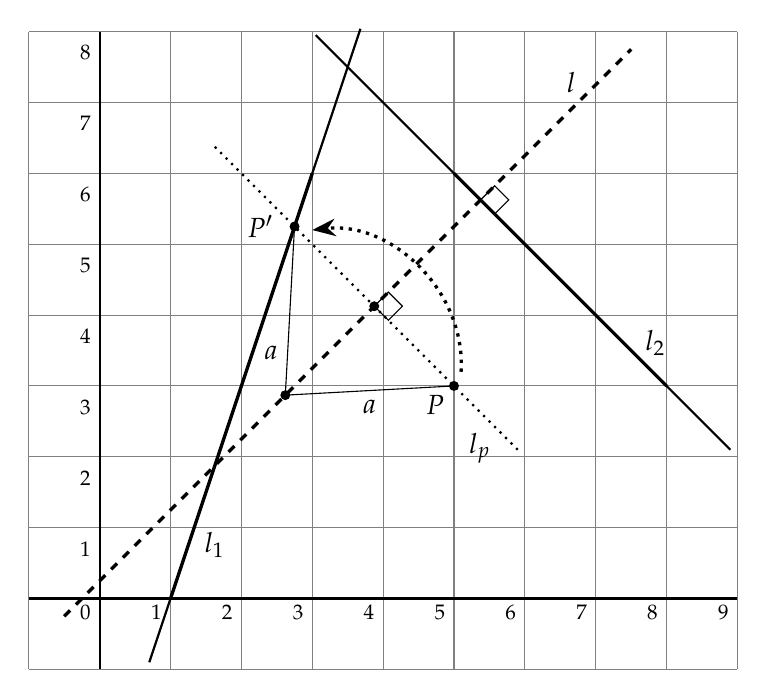
\begin{tikzpicture}[scale=.9]
\draw[step=10mm,white!50!black,thin] (-1,-1) grid (9,8);
\draw[thick] (-1,0) -- (9,0);
\draw[thick] (0,-1) -- (0,8);
\foreach \x in {0,...,9}
  \node at (\x-.2,-.2) {\sm{\x}};
\foreach \y in {1,...,8}
  \node at (-.2,\y-.3) {\sm{\y}};
\coordinate (P1) at (5,3);
\fill (P1) circle (2pt) node[below left] {$P$};
\coordinate (P1P) at (2.75,5.25);
\fill (P1P) circle (2pt) node[left,xshift=-4pt] {$P'$};
\draw[very thick] (1,0) -- node[very near start,right,xshift=2pt] {$l_1$} (3,6);
\draw[very thick,name path=l2] (8,3) -- node[very near start,right,xshift=-2pt,yshift=6pt] {$l_2$} (5,6);
\draw[thick] ($(1,0)!-.15!(3,6)$) -- ($(1,0)!1.34!(3,6)$);
\draw[thick] ($(8,3)!-.3!(5,6)$) -- ($(8,3)!1.65!(5,6)$);
\draw[thick,dotted] ($(P1)!-.4!(P1P)$) -- node[very near start,below,yshift=-4pt] {$l_p$} ($(P1)!1.5!(P1P)$);
\draw[very thick,dashed,name path=fold] (-.5,-.25) -- node[very near end,above,xshift=4pt,yshift=6pt] {$l$} (7.5,7.75);
\coordinate(a) at ($(-.5,-.25)!.39!(7.5,7.75)$);
\fill (a) circle (2pt);
\draw (P1) -- node[below] {$a$} (a) -- node[left,near start] {$a$} (P1P);
\coordinate (mid) at ($(P1)!.5!(P1P)$);
\fill (mid) circle (2pt);
\path [name intersections = {of = fold and l2, by = {perp}}];
\draw[rotate=-45] (mid) rectangle +(8pt,8pt);
\draw[rotate=-45] (perp) rectangle +(8pt,8pt);
\draw[very thick,dotted,->,bend right=50] (5.1,3.2) to (3,5.2);
\end{tikzpicture}
\end{center}


\tikzsetfigurename{exercises}
% !TeX root = origami-activities-en.tex

%%%%%%%%%%%%%%%%%%%%%%%%%%%%%%%%%%%%%%%%%%%%%%%%%%%%%%%%%%%%%%%%%%
%%%%%%%%%%%%%%%%%%%%%%%%%%%%%%%%%%%%%%%%%%%%%%%%%%%%%%%%%%%%%%%%%%
%%%%%%%%%%%%%%%%%%%%%%%%%%%%%%%%%%%%%%%%%%%%%%%%%%%%%%%%%%%%%%%%%%

\section{Exercises for geometric loci}\label{s.exercises}

The following exercises are rather basic and can be integrated into the activities or used to summarize the activities. Some of them can be solved using algebra alone, but insights from origami can deepened the students' understanding of the axioms.

\begin{enumerate}
\item Find the geometric locus of all the points whose distance from the point $(-8,-6)$ is equal to their distances from $(12,4)$.

\item Find the geometric locus of all the points whose sum or difference of their distances from $P_1=(2,3)$ and $P_2=(6,4)$ is equal to the length of the line segment $\overline{P_1P_2}$.

\item 
\begin{enumerate}
\item Find the geometric locus of all the points whose distance from the line $5x+3y-14=0$ is equal to their distance to the line $3x+5y-34=0$.
\item What is the form of the geometric locus that you found?
\item Explain why all the lines you found in the previous items bisect the angle between the two given lines.
\end{enumerate}

\item Find the geometric locus of all points whose distance from the line $y=2x+6$ is equal to the distance from the line $y=2x-4.5$.

\item 
\begin{enumerate} 
\item Find the geometric locus of all the points whose distance from the point $(3,-6)$ is $9$.
\item What is the form of the geometric locus that you found?
\end{enumerate}

\item Find the geometric locus of all the points on the line $y=x+1$ whose distance from the point $(2,10)$ is $5$.

\item
\begin{enumerate}
\item What is the form of the geometric locus of all points whose distance from the point $(0,3)$ is equal to their distance from the line $y=-3$.
\item What is the geometric locus?
\end{enumerate}

\end{enumerate}


\tikzsetfigurename{appendix1}
% !TeX root = origami-activities-en.tex

\appendix

\section{Experiments with the origami axioms}\label{a.experimenting}

% Axiom 1
\begin{wrapfigure}[4]{r}{.4\textwidth}
\begin{center}
\vspace{-4ex}
\begin{tikzpicture}[scale=.9]
\coordinate (P1) at (3,6);
\coordinate (P2) at (4,3);
\fill (P1) circle (1.5pt) node[below left] {$P_1$};
\fill (P2) circle (1.5pt) node[below left] {$P_2$};
\draw[thick,dashed] ($(P1)!-.2!(P2)$) -- ($(P1)!1.5!(P2)$);
\draw[very thick,dotted,->,bend left=35] (5,5) to (2,4);
\end{tikzpicture}
\end{center}
\end{wrapfigure}
\textbf{Axiom $1$} Given two points $P_1,P_2$, there is a single fold that passes through them.

Task: Label two arbitrary points on a sheet of paper. Fold the paper so that the fold pass through the two labeled points.

\vspace{14ex}

\begin{wrapfigure}[4]{r}{.4\textwidth}
% Axiom 2
\begin{center}
\vspace{-4ex}
\begin{tikzpicture}[scale=.8]
\coordinate (P1) at (3,5);
\coordinate (P2) at (5,1);
\fill (P1) circle (1.5pt) node[above left] {$P_1$};
\fill (P2) circle (1.5pt) node[below right] {$P_2$};
\draw[thick,dashed] (2,2) -- (7,4);
\draw[very thick,dotted,->,bend left=35] (3.2,4.8) to (5,1.2);
\end{tikzpicture}
\end{center}
\end{wrapfigure}
\textbf{Axiom $2$} Given two points $P_1,P_2$, there is a single fold that places $P_1$ onto $P_2$.

Task: Label two arbitrary points on a sheet of paper. Fold the paper so that one point is placed on top of the other.

\vspace{16ex}


\begin{wrapfigure}[4]{r}{.4\textwidth}
% Axiom 3
\begin{center}
\vspace{-4ex}
\begin{tikzpicture}[scale=.8]
\draw (1,2) -- node[near start,above,xshift=-4pt] {$l_1$} (3,6);
\draw (2,1) -- node[near start,below] {$l_2$} (8,4);
\draw[thick,dashed] (1,1) -- (6,6);
\draw[very thick,dotted,->,bend left=35] (2.2,4.2) to (3.9,2.1);
\end{tikzpicture}
\end{center}
\end{wrapfigure}
\textbf{Axiom $3$} Given two lines $l_1,l_2$, there is a fold that places $l_1$ onto $l_2$.

Task: Draw two arbitrary intersecting lines on a sheet of paper. Fold the paper so that one line is placed onto the other. Is there more than one fold that can do this?

\vspace{14ex}

% Axiom 4
\begin{wrapfigure}[4]{r}{.4\textwidth}
\begin{center}
\vspace{-4ex}
\begin{tikzpicture}[scale=.9]
\coordinate (L1a) at (3,2);
\coordinate (L1b) at (5,6);
\draw[thick] (L1a) -- node[very near start,right,yshift=-4pt] {$l$} ($(L1a)!1.15!(L1b)$);
\fill (3,5.5) circle (2pt) node[above right] {$P$};
\draw[thick,dashed] (2,6) -- (8,3);
\coordinate (intersection) at (4.4,4.8);
\draw[rotate=-30] (intersection) rectangle +(8pt,8pt);
\draw[very thick,dotted,->,bend left=50] (5.4,6.3) to (3.7,3);
\end{tikzpicture}
\end{center}
\end{wrapfigure}
\textbf{Axiom $4$} Given a point $P$ and a line $l$, there is a single fold perpendicular to $l$ that passes through $P$.

Task: Draw an arbitrary line and an arbitrary point on a sheet of paper. Fold the paper so that the fold passes through the point and is perpendicular to the line.

\newpage

\begin{wrapfigure}[5]{r}{.4\textwidth}
% Axiom 5
\begin{center}
\vspace{-3ex}
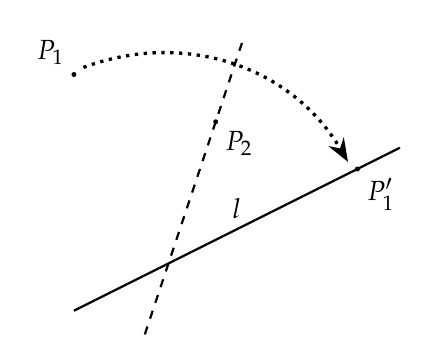
\begin{tikzpicture}[scale=.6]
\coordinate (P1) at (1,4);
\coordinate (P2) at (4,3);
\fill (P1) circle (1.5pt) node[above left] {$P_1$};
\fill (P2) circle (1.5pt) node[below right] {$P_2$};
\draw[thick,dashed] (2.5,-1.5) -- (4.6,4.8); %($(3,0)!-.15!(5,6)$) -- (5,6);
\draw[thick] (1,-1) -- node[above] {$l$} ($(1,-1)!1.15!(7,2)$);
\coordinate (P3) at (7,2);
\fill (P3) circle (1.5pt) node[below right] {$P_1'$};
\draw[->,very thick,dotted,bend left=40] ($(P1)+(.2,.15)$) to ($(P3)+(-.2,.15)$);
\end{tikzpicture}
\end{center}
\end{wrapfigure}

\textbf{Axiom $5$} Given two points $P_1,P_2$ and a line $l$, there is a fold that places $P_1$ onto $l$ and passes through $P_2$.

Task: Draw two arbitrary points and an arbitrary line on a sheet of paper. Fold the paper so that the fold passes through one point and places the other point on the line.

\vspace{14ex}

\begin{wrapfigure}[8]{r}{.4\textwidth}
% Axiom 6
\begin{center}
\vspace{-6ex}
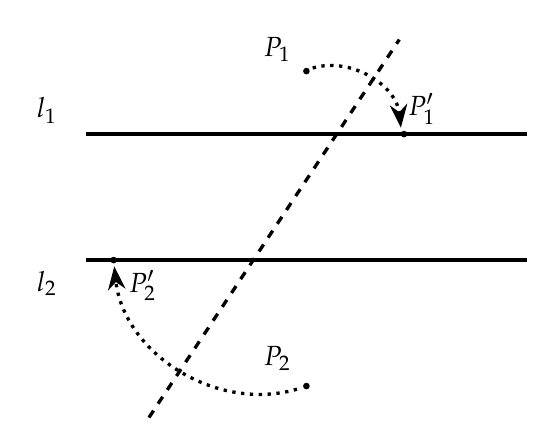
\begin{tikzpicture}[scale=.4]
\coordinate (P1) at (0,4);
\fill (P1) circle (3pt) node[above left,xshift=-2pt] {$P_1$};
\coordinate (P2) at (0,-6);
\fill (P2) circle (3pt) node[above left,xshift=-2pt,yshift=2pt] {$P_2$};
\coordinate (P1P) at (3.1,2);
\fill (P1P) circle (3pt) node[above right,xshift=-2pt] {$P_1'$};
\coordinate (P2P) at (-6.12,-2);
\fill (P2P) circle (3pt) node[below right,xshift=2pt] {$P_2'$};
\draw[very thick] (-7,2) -- node[very near start,above,xshift=-34pt] {$l_1$} (7,2);
\draw[very thick] (-7,-2) -- node[very near start,below,xshift=-34pt] {$l_2$} (7,-2);
\draw[very thick,dashed] (-5,-7) -- (2.95,5);
\draw[very thick,dotted,->,bend left=50] (.2,4.1) to (3,2.2);
\draw[very thick,dotted,->,bend left=50] (-.3,-6.1) to (-6.1,-2.2);
\end{tikzpicture}
\end{center}
\end{wrapfigure}

\textbf{Axiom $6$} Given two points $P_1,P_2$ and two lines $l_1,l_2$, there is a fold that simultaneously places $P_1$ onto $l_1$ and $P_2$ onto $l_2$.

Task: Draw two arbitrary points and two arbitrary lines on a sheet of paper. Fold the paper so that each point is one of the lines.

\vspace{16ex}

\begin{wrapfigure}{r}{.4\textwidth}
% Axiom 7
\begin{center}
\vspace{-8ex}
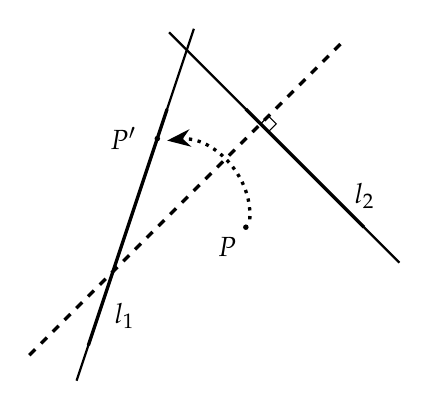
\begin{tikzpicture}[scale=.5]
\coordinate (P1) at (5,3);
\fill (P1) circle (2pt) node[below left] {$P$};
\coordinate (P1P) at (2.75,5.25);
\fill (P1P) circle (2pt) node[left,xshift=-4pt] {$P'$};
\draw[very thick] (1,0) -- node[very near start,right,xshift=2pt] {$l_1$} (3,6);
\draw[very thick,name path=l2] (8,3) -- node[very near start,right,xshift=-2pt,yshift=6pt] {$l_2$} (5,6);
\draw[thick] ($(1,0)!-.15!(3,6)$) -- ($(1,0)!1.34!(3,6)$);
\draw[thick] ($(8,3)!-.3!(5,6)$) -- ($(8,3)!1.65!(5,6)$);
\draw[very thick,dashed,name path=fold] (-.5,-.25) -- (7.5,7.75);
\path [name intersections = {of = fold and l2, by = {perp}}];
\draw[rotate=-45] (perp) rectangle +(8pt,8pt);
\draw[very thick,dotted,->,bend right=50] (5.1,3.2) to (3,5.2);
\end{tikzpicture}
\end{center}
\end{wrapfigure}
\textbf{Axiom $7$} Given a point $P$ and two lines $l_1,l_2$, there is a fold that places $P$ onto $l_1$ and is perpendicular to $l_2$.

Task: Draw an arbitrary point and two arbitrary lines on a sheet of paper. Fold the paper so the point is placed onto one of the lines and the fold is perpendicular to the other line.
\tikzsetfigurename{appendix2}
% !TeX root = origami-activities-en.tex


%%%%%%%%%%%%%%%%%%%%%%%%%%%%%%%%%%%%%%%%%%%%%%%%%%%%%%%%%%%%%%%%%%
%%%%%%%%%%%%%%%%%%%%%%%%%%%%%%%%%%%%%%%%%%%%%%%%%%%%%%%%%%%%%%%%%%
%%%%%%%%%%%%%%%%%%%%%%%%%%%%%%%%%%%%%%%%%%%%%%%%%%%%%%%%%%%%%%%%%%


\section{The number of common tangents to two parabolas}\label{a.parabola}

The following diagrams that two parabolas can have zero, one, two or three common tangents.

\bigskip

\begin{center}
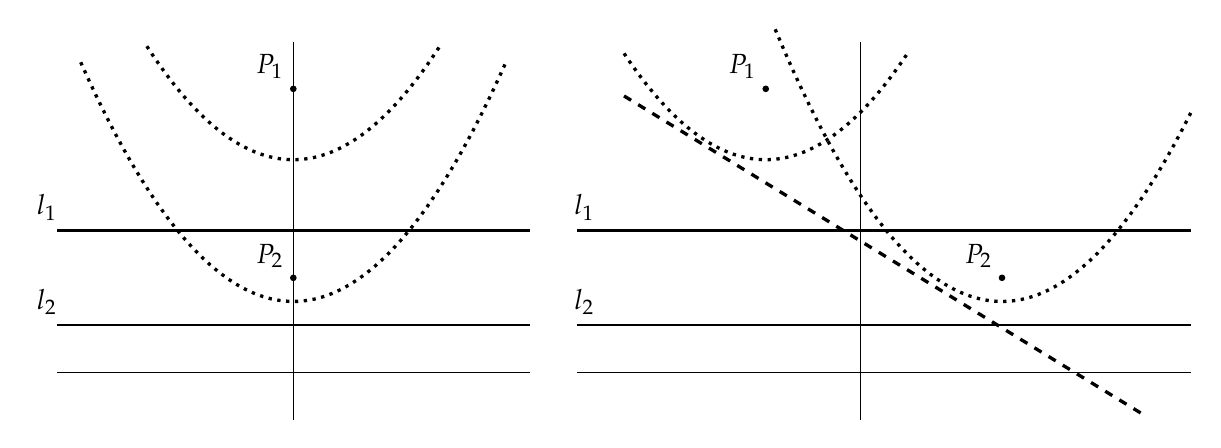
\begin{tikzpicture}[scale=.6]
\draw (-5,0) -- (5,0);
\draw (0,-1) -- (0,7);
\coordinate (P1) at (0,6);
\fill (P1) circle (2pt) node[above left] {$P_1$};
\coordinate (P2) at (0,2);
\fill (P2) circle (2pt) node[above left] {$P_2$};
\draw[thick] (-5,3) -- node[very near start,above,xshift=-25pt] {$l_1$} (5,3);
\draw[thick] (-5,1) -- node[very near start,above,xshift=-25pt] {$l_2$} (5,1);
\draw[domain=-3.1:3.1,samples=50,very thick,dotted] plot (\x,{.25*\x*\x+4.5});
\draw[domain=-4.5:4.5,samples=50,very thick,dotted] plot (\x,{.25*\x*\x+1.5});
\begin{scope}[xshift=12cm]
\draw (-6,0) -- (7,0);
\draw (0,-1) -- (0,7);
\coordinate (P1) at (-2,6);
\fill (P1) circle (2pt) node[above left] {$P_1$};
\coordinate (P2) at (3,2);
\fill (P2) circle (2pt) node[above left] {$P_2$};
\draw[thick] (-6,3) -- node[very near start,above,xshift=-25pt] {$l_1$} (7,3);
\draw[thick] (-6,1) -- node[very near start,above,xshift=-25pt] {$l_2$} (7,1);
\draw[domain=-5:1,samples=50,very thick,dotted] plot (\x,{.25*(\x+2)*(\x+2)+4.5});
\draw[domain=-1.8:7,samples=50,very thick,dotted] plot (\x,{.25*(\x-3)*(\x-3)+1.5});
\draw[very thick,dashed] (-5,5.85) -- (6,-.9);
\end{scope}
\end{tikzpicture}
\end{center}

\bigskip
\bigskip
\bigskip

%\begin{center}
%
%\begin{tikzpicture}[scale=.6]
%\draw (-7,0) -- (7,0);
%\draw (0,-1) -- (0,7);
%\coordinate (P1) at (-2,6);
%\fill (P1) circle (2pt) node[above left] {$P_1$};
%\coordinate (P2) at (3,2);
%\fill (P2) circle (2pt) node[above left] {$P_2$};
%\draw[thick] (-7,3) -- node[very near start,above,xshift=-25pt] {$l_1$} (7,3);
%\draw[thick] (-7,1) -- node[very near start,above,xshift=-25pt] {$l_2$} (7,1);
%\draw[domain=-5:1,samples=50,very thick,dotted] plot (\x,{.25*(\x+2)*(\x+2)+4.5});
%\draw[domain=-1.8:7,samples=50,very thick,dotted] plot (\x,{.25*(\x-3)*(\x-3)+1.5});
%\draw[very thick,dashed] (-5,5.85) -- (6,-.9);
%\end{tikzpicture}
%\end{center}
%
%\bigskip\bigskip
%

\begin{center}
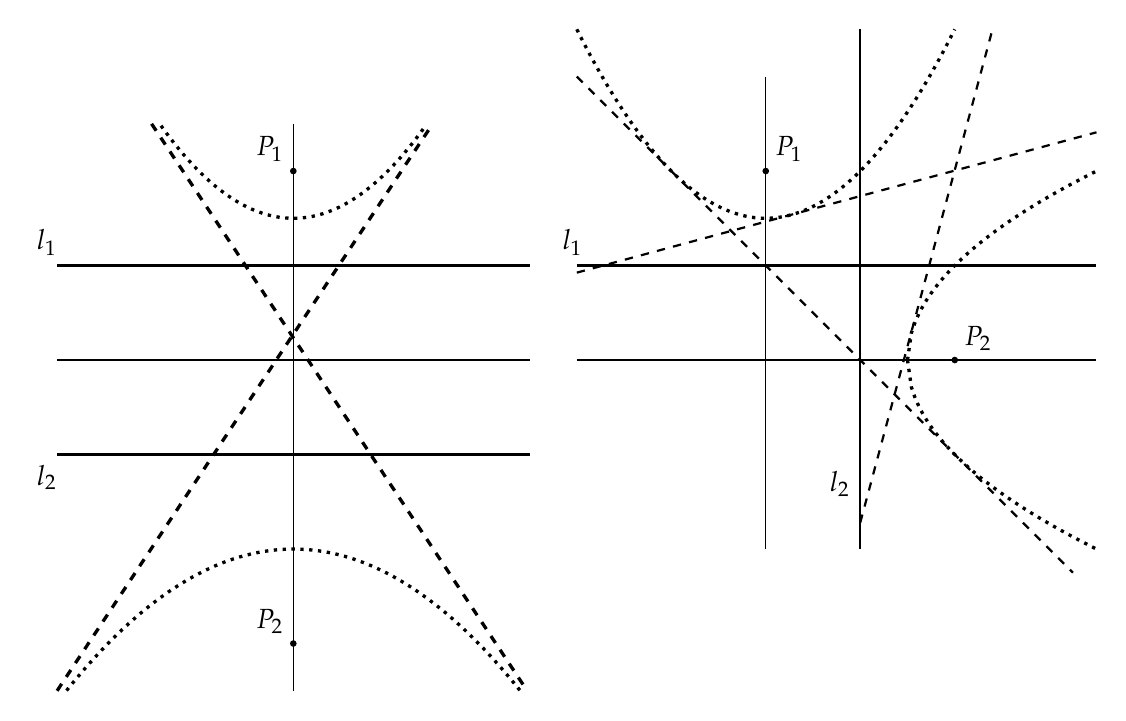
\begin{tikzpicture}[scale=.6]
\draw (-5,0) -- (5,0);
\draw (0,-7) -- (0,5);
\coordinate (P1) at (0,4);
\fill (P1) circle (2pt) node[above left] {$P_1$};
\coordinate (P2) at (0,-6);
\fill (P2) circle (2pt) node[above left] {$P_2$};
\draw[thick] (-5,2) -- node[very near start,above,xshift=-25pt] {$l_1$} (5,2);
\draw[thick] (-5,-2) -- node[very near start,below,xshift=-25pt] {$l_2$} (5,-2);
\draw[domain=-4.8:4.8,samples=50,very thick,dotted] plot (\x,{-.13*\x*\x-4});
\draw[domain=-2.8:2.8,samples=50,very thick,dotted] plot (\x,{.25*\x*\x+3});
\draw[very thick,dashed] (-5,-7) -- (2.95,5);
\draw[very thick,dashed] (-3,5) -- (4.95,-7);
\begin{scope}[xshift=10cm]
\draw (-4,0) -- (7,0);
\draw (0,-4) -- (0,6);
\coordinate (P1) at (0,4);
\fill (P1) circle (2pt) node[above right] {$P_1$};
\coordinate (P2) at (4,0);
\fill (P2) circle (2pt) node[above right] {$P_2$};
\draw[thick] (-4,2) -- node[very near start,above,xshift=-25pt] {$l_1$} (7,2);
\draw[thick] (2,-4) -- node[very near start,left] {$l_2$} (2,7);
\draw[domain=-4:4,samples=50,very thick,dotted] plot (\x,{.25*\x*\x+3});
\draw[domain=3:7,samples=50,very thick,dotted] plot (\x,{sqrt(4*\x-12)});
\draw[domain=3:7,samples=50,very thick,dotted] plot (\x,{-sqrt(4*\x-12)});

\draw[thick,dashed,domain=-4:6.5] plot (\x,-\x+2);
\draw[thick,dashed,domain=-4:7] plot (\x,.27*\x+2.93);
\draw[thick,dashed,domain=2:4.8] plot (\x,3.73*\x-10.9);
\end{scope}
\end{tikzpicture}
\end{center}

%\begin{center}
%\begin{tikzpicture}[scale=.6]
%\draw (-4,0) -- (7,0);
%\draw (0,-4) -- (0,6);
%\coordinate (P1) at (0,4);
%\fill (P1) circle (2pt) node[above right] {$P_1$};
%\coordinate (P2) at (4,0);
%\fill (P2) circle (2pt) node[above right] {$P_2$};
%\draw[thick] (-4,2) -- node[very near start,above,xshift=-25pt] {$l_1$} (7,2);
%\draw[thick] (2,-4) -- node[very near start,left] {$l_2$} (2,7);
%\draw[domain=-4:4,samples=50,very thick,dotted] plot (\x,{.25*\x*\x+3});
%\draw[domain=3:7,samples=50,very thick,dotted] plot (\x,{sqrt(4*\x-12)});
%\draw[domain=3:7,samples=50,very thick,dotted] plot (\x,{-sqrt(4*\x-12)});
%
%\draw[thick,dashed,domain=-4:6.5] plot (\x,-\x+2);
%\draw[thick,dashed,domain=-4:7] plot (\x,.27*\x+2.93);
%\draw[thick,dashed,domain=2:4.8] plot (\x,3.73*\x-10.9);
%\end{tikzpicture}
%\end{center}

\tikzsetfigurename{appendix3}
% !TeX root = origami-activities-en.tex

%%%%%%%%%%%%%%%%%%%%%%%%%%%%%%%%%%%%%%%%%%%%%%%%%%%%%%%%%%%%%%%%%%
%%%%%%%%%%%%%%%%%%%%%%%%%%%%%%%%%%%%%%%%%%%%%%%%%%%%%%%%%%%%%%%%%%
%%%%%%%%%%%%%%%%%%%%%%%%%%%%%%%%%%%%%%%%%%%%%%%%%%%%%%%%%%%%%%%%%%

\section{Solutions to the exercises in Section~\ref{s.exercises}}

\textbf{Question 1} Find the geometric locus of all the points whose distance from the point $(-8,-6)$ is equal to their distances from $(12,4)$.

\textbf{Solution}

The geometric locus of all points equidistant from $P_1$ and $P_2$ is the perpendicular bisector of the segment $\overline{P_1P_2}$. Let us find the equation of the perpendicular bisector of the segment connecting $(-8,-6)$ and $(12,4)$. The slope is the negative inverse of the segment, which is $-2$ since the slope of the segment is:
\[
\disfrac{4-(-6)}{12-(-8)}=\disfrac{1}{2}\,.
\]
The midpoint of $\overline{P_1P_2}$ is:
\[
\left(\disfrac{-8+12}{2},\disfrac{-6+4}{2}\right)=(2,-1)\,.
\]
The equation of the perpendicular bisector is:
\begin{form}{1}
y-(-1)&=&-2(x-2)\\
y&=&-2x+3\,.
\end{form}

\textbf{Question 2} Find the geometric locus of all points whose sum or difference of their distances from $P_1=(2,3)$ and $P_2=(6,4)$ is equal to the length of the line segment $\overline{P_1P_2}$. 

\textbf{Solution} In Activity 3 we saw that the geometric locus of all points whose sum or difference of their distance from $P_1$ and $P_2$ is equal to the length of $\overline{P_1P_2}$ is the line that passes through $P_1$ and $P_2$.

The slope is:
\[
\disfrac{4-3}{6-2}=\disfrac{1}{4}\,,
\]
so the equation of the line is:
\begin{form}{2}
y-3&=&\disfrac{1}{4}(x-2)\\
y&=&\disfrac{2}{3}(x + 1)\,.
\end{form}

\textbf{Question 3}
\begin{enumerate}
\item Find the geometric locus of all points whose distance from the line $5x+3y-14=0$ is equal to their distance to the line $3x+5y-34=0$.
\item What is the form of the geometric locus that you found?
\item Explain why all the lines you found in the previous items bisect the angle between the two given lines.
\end{enumerate}

\textbf{Solution}

\textbf{(1)} Let $(x,y)$ be any point that satisfies the condition. We will use the formula for finding the distance of a point from a line in the plane. We do this for each line and then equate them. The distance of $(x,y)$ from $5x+3y-14$ is:
\[
\left|\disfrac{5x+3y-14}{\sqrt{5^2+3^2}}\right|=\left|\disfrac{5x+3y-14}{\sqrt{34}}\right|\,.
\]
The distance of $(x,y)$ from $3x+5y-34$ is:
\[
\left|\disfrac{3x+5y-34}{\sqrt{3^2+5^2}}\right|=\left|\disfrac{3x+5y-34}{\sqrt{34}}\right|\,.
\]
Equating the formulas and multiplying by $\sqrt{34}$:
\[
|5x+3y-14|=|3x+5y-34|\,.
\]
There are two cases depending on the signs:
\begin{form}{1}
5x+3y-14&=&3x+5y-34\\
x-y+10&=&0\,,
\end{form}
and
\begin{form}{1}
5x+3y-14&=&-(3x+5y-34)\\
x+y-6&=&0\,.
\end{form}

\textbf{(2)} The geometric locus is two lines.

\textbf{(3)} This was proved in the Activity.


\textbf{Question 4}  Find the geometric locus of all points whose distance from the line $y=2x+6$ is equal to the distance from the line $y=2x-4.5$.

\textbf{Solution}

Both of the given lines have the same slope so they are parallel. We saw that when two lines are parallel, the geometric locus of the points equidistant from them is the line parallel to them and equidistant from them. 

The line with have an equation of the form $-2x-y+c=0$. Since it is equidistant from them, we use the equation for the distance between two parallel lines and equate them:
\[
\disfrac{|6-c|}{\sqrt{(-2)^2+(-1)^2}}=\disfrac{|-4.5-c|}{\sqrt{(-2)^2+(-1)^2}}\,.
\]
It follows that:
\[
|6-c|=|-4.5-c|\,,
\]
so the equation has the single solution $c=\disfrac{3}{4}$ and the line of the equation is $-2x-y-\disfrac{3}{4}$.

\newpage

\textbf{Question 5}
\begin{enumerate} 
\item Find the geometric locus of all the points whose distance from the point $(3,-6)$ is $9$.
\item What is the form of the geometric locus that you found?
\end{enumerate}

\textbf{Solution}

\textbf{(1)} Let $(x,y)$ be any point that satisfies the condition. We will use the formula for finding the distance between two points:
\begin{form}{1.3}
9&=&\sqrt{(x-3)^2+(y+6)^2}\\
81&=&(x-3)^2+(y+6)^2\,.
\end{form}

\textbf{(2)} The geometric locus is a circle.

\textbf{Question 6}  Find the geometric locus of all points on the line $y=x+1$ whose distance from the point $(2,10)$ is $5$.

\textbf{Solution} The geometric locus of all points whose distance from $(2,10)$ is $5$ is a circle whose equation is $(x-2)^2+(y-10)^2=25$. We saw that the geometric locus that we seek is the point or points of intersection of the line with the circle. Substitute the equation for the line into the equation of the circle:
\begin{form}{1.5}
(x-2)^2+((x+1)-10)^2&=&25\\
(x-2)^2+(x-9)^2&=&25\\
x^2-4x+4+x^2-18x+81&=&25\\
2x^2-22x+60&=&0\\
x=&=&5,\;6\,.
\end{form}
By substituting these values into the equation for the line we obtain that the two points of intersection are $(6,7),\:(5,6)$.

\textbf{Question $7$} 
\begin{enumerate}
\item What is the form of the geometric locus of all point whose distance from the point $(0,3)$ is equal to their distance from the line $y=-3$.
\item What is the geometric locus?
\end{enumerate}


\textbf{Solution}

\textbf{(1)} The geometric locus is a parabola whose focus is $(0,3)$ and whose directrix is $y=-3$.

\textbf{(2)} We use the formula for the equation of a parabola:
\begin{form}{1}
x^2=4\cdot 3y\\
x^2&=&12y\,.
\end{form}



\tikzsetfigurename{appendix4}
% !TeX root = origami-activities-en.tex
\section{Geogebra constructions for the origami axioms}

%%%%%%%%%%%%%%%%%%%%%%%%%%%%%%%%%%%%%%%%%%%%%%%%%%%%%%%%%%%%%%%%%%
%%%%%%%%%%%%%%%%%%%%%%%%%%%%%%%%%%%%%%%%%%%%%%%%%%%%%%%%%%%%%%%%%%
%%%%%%%%%%%%%%%%%%%%%%%%%%%%%%%%%%%%%%%%%%%%%%%%%%%%%%%%%%%%%%%%%%

The italicized words refer to menu selections in Geogebra.

\textbf{Axiom $1$} Construct two \emph{points}. Construct a \emph{line} throught the points.

\textbf{Axiom $2$} Construct two \emph{points}. Construct the \emph{perpendicular bisector} of the line \emph{segment} connecting the two points. Construct the \emph{reflection} of one point relative to the line to check that it is placed on the other point.

\textbf{Axiom $3$} For the case where $l_1,l_2$ intersect: construct two \emph{segments} that intersect or that would intersect if extended. Construct the \emph{angle bisector} between the segments. (You can extend the segments so that they intersect but that is not necessary.) Construct the \emph{reflection} of one line relative to the bisector and check if it is placed on the other line. (You can change the color of one line to make it clear that they are placed on each other.)

For the case where $l_1,l_2$ are parallel: construct two parallel \emph{segments}. Construct a \emph{perpendicular} to one segment and construct its \emph{intersection} with the second segment (extended if necessary). Construct the \emph{perpendicular bisector} of the segment between between the two lines. Construct the \emph{reflection} of one line relative to the bisector and check that it is placed on the other line. (You can change the color of one line to make it clear that they are placed on each other.)

\textbf{Axiom $4$} Construct a \emph{line} and a \emph{point} not on the line. Construct a \emph{perpendicular} to the line through the point. Construct a \emph{reflection} of some point on the line relative to the perpendicular to check that it is placed on the line.

\textbf{Axiom $5$} Construct a \emph{line} $l$ and \emph{points} $P_1,P_2$. Construct a \emph{circle through point $P_1$} with center $P_2$. Construct the \emph{intersections} $A,B$ of $l$ and the circle. Construct line \emph{segments} $\overline{P_1A}, \overline{P_1B}$. Construct a \emph{perpendiculars} through $P_2$ those segments. Construct a \emph{reflection} of $P_1$ relative to one of the perpendiculars to check that it is placed on the line. Repeat with the other perpendicular.

\textbf{Axiom $6$} Construct two \emph{lines} $l_1,l_2$ and two \emph{points} $P_1,P_2$. Construct a \emph{parabola} with focus $P_1$ and directrix $l_1$ and \emph{parabola} with focus $P_2$ and directrix $l_2$. Construct \emph{tangents} to both parabolas. Construct the \emph{reflections} of $P_1,P_2$ relative to one of the tangents and check that they are placed on the lines $l_1,l_2$.

\textbf{Axiom $7$} Construct two line \emph{segments} $l_1,l_2$ and a \emph{point} $P$. Construct a \emph{parallel} to $l_2$ through $p$, and construct $P_1'$, the \emph{intersection} of the parallel and $l_1$. (Extend $l_1$ if necessary.) Construct the  \emph{segment} $\overline{PP'}$ and construct its \emph{perpendicular bisector}. Construct the \emph{reflection} of $P$ relative to the bisector and check that it is placed on $P'$.

% !TeX root = origami-activities-en.tex

%%%%%%%%%%%%%%%%%%%%%%%%%%%%%%%%%%%%%%%%%%%%%%%%%%%%%%%%%%%%%%%%%%
%%%%%%%%%%%%%%%%%%%%%%%%%%%%%%%%%%%%%%%%%%%%%%%%%%%%%%%%%%%%%%%%%%
%%%%%%%%%%%%%%%%%%%%%%%%%%%%%%%%%%%%%%%%%%%%%%%%%%%%%%%%%%%%%%%%%%

\section*{Further reading}

Applications of origami \cite{lang-ted}. Mathematical theory of origami \cite{alperin,moti-origami}. History of origami \cite{history}. Paper folding \cite{lang,newton}.


\bibliographystyle{plain}
\bibliography{origami-activities-en}

\end{document}
	